\documentclass[10pt]{beamer}

\usetheme[progressbar=frametitle]{metropolis}
\usepackage{appendixnumberbeamer}

\usepackage{booktabs}
\usepackage[scale=2]{ccicons}

\usepackage{pgfplots}
\usepgfplotslibrary{dateplot}

\usepackage{xspace}
\newcommand{\themename}{\textbf{\textsc{metropolis}}\xspace}

\title{Uni- and Multivariate Analysis of Dendritic Ca2+ Data}
\subtitle{In a Stimulus Detection Task}
\date{\today}
%\date{}
\author{Georg Chechelnizki}
\institute{BCCN Berlin}
% \titlegraphic{\hfill\includegraphics[height=1.5cm]{logo.pdf}}

\setbeamercolor{background canvas}{bg=white}
\usepackage{caption}

\begin{document}

\maketitle

\begin{frame}{Table of contents}
  \setbeamertemplate{section in toc}[sections numbered]
  \tableofcontents[hideallsubsections]
\end{frame}

\section{Introduction}

\begin{frame}[fragile]{The Experiment}
\begin{columns}[T,onlytextwidth]
    \column{0.5\textwidth}
    	\only<+->{
      \begin{figure}
      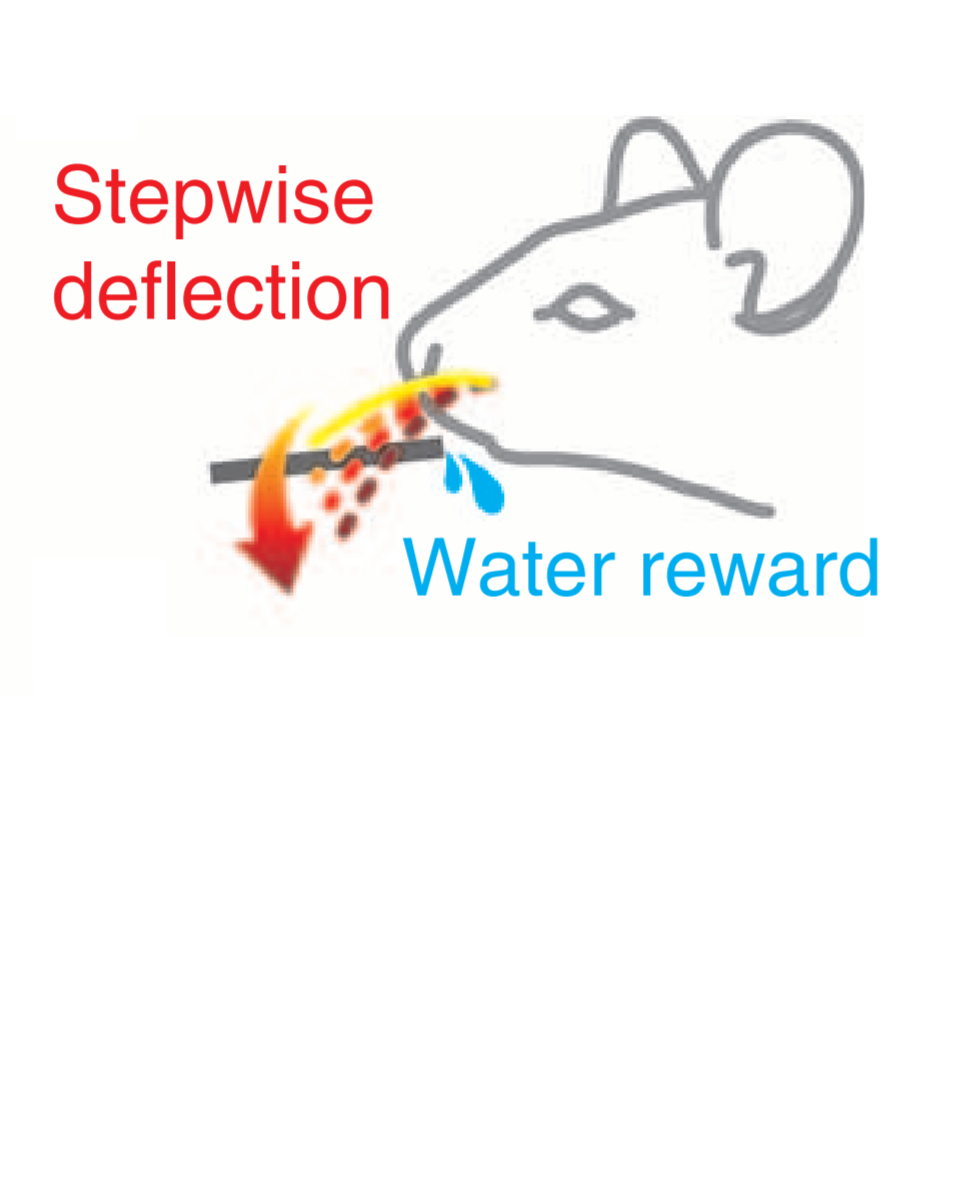
\includegraphics[scale=0.1]{mouse.png}
      \end{figure}}
      
    \column{0.5\textwidth}
		\only<+->{
      \begin{figure}
      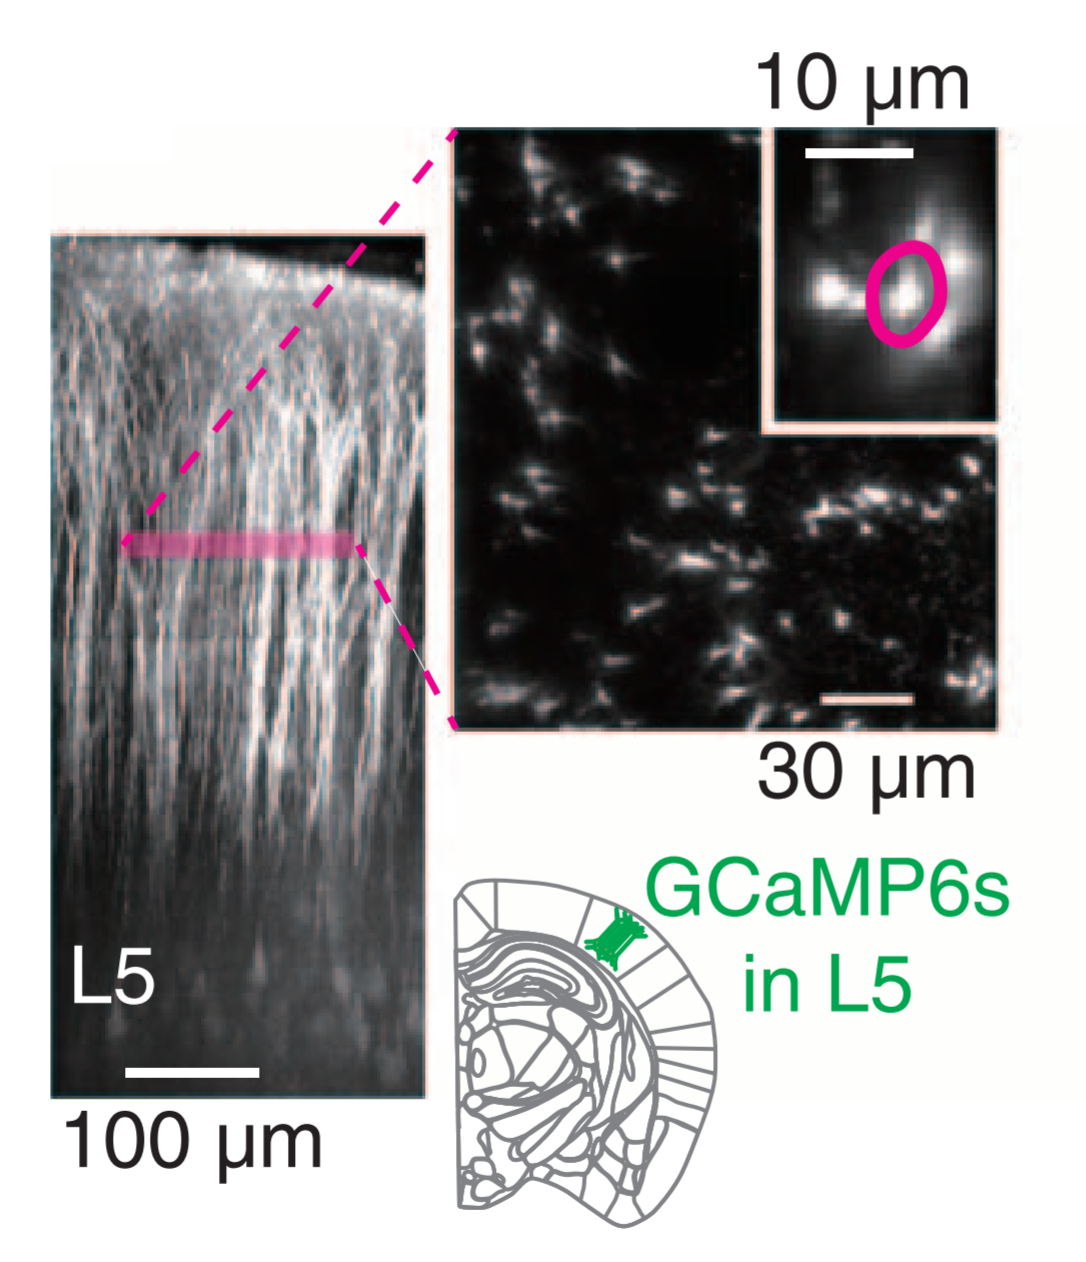
\includegraphics[scale=0.1]{roi.png}
      \end{figure}}

  \end{columns}
\end{frame}

\begin{frame}[fragile]{The Data - Neuronal}
	\begin{center}
	\begin{figure}
	\caption*{Trial-averaged $\text{Ca}^{2+}$ fluorescence traces of random dendrites}
      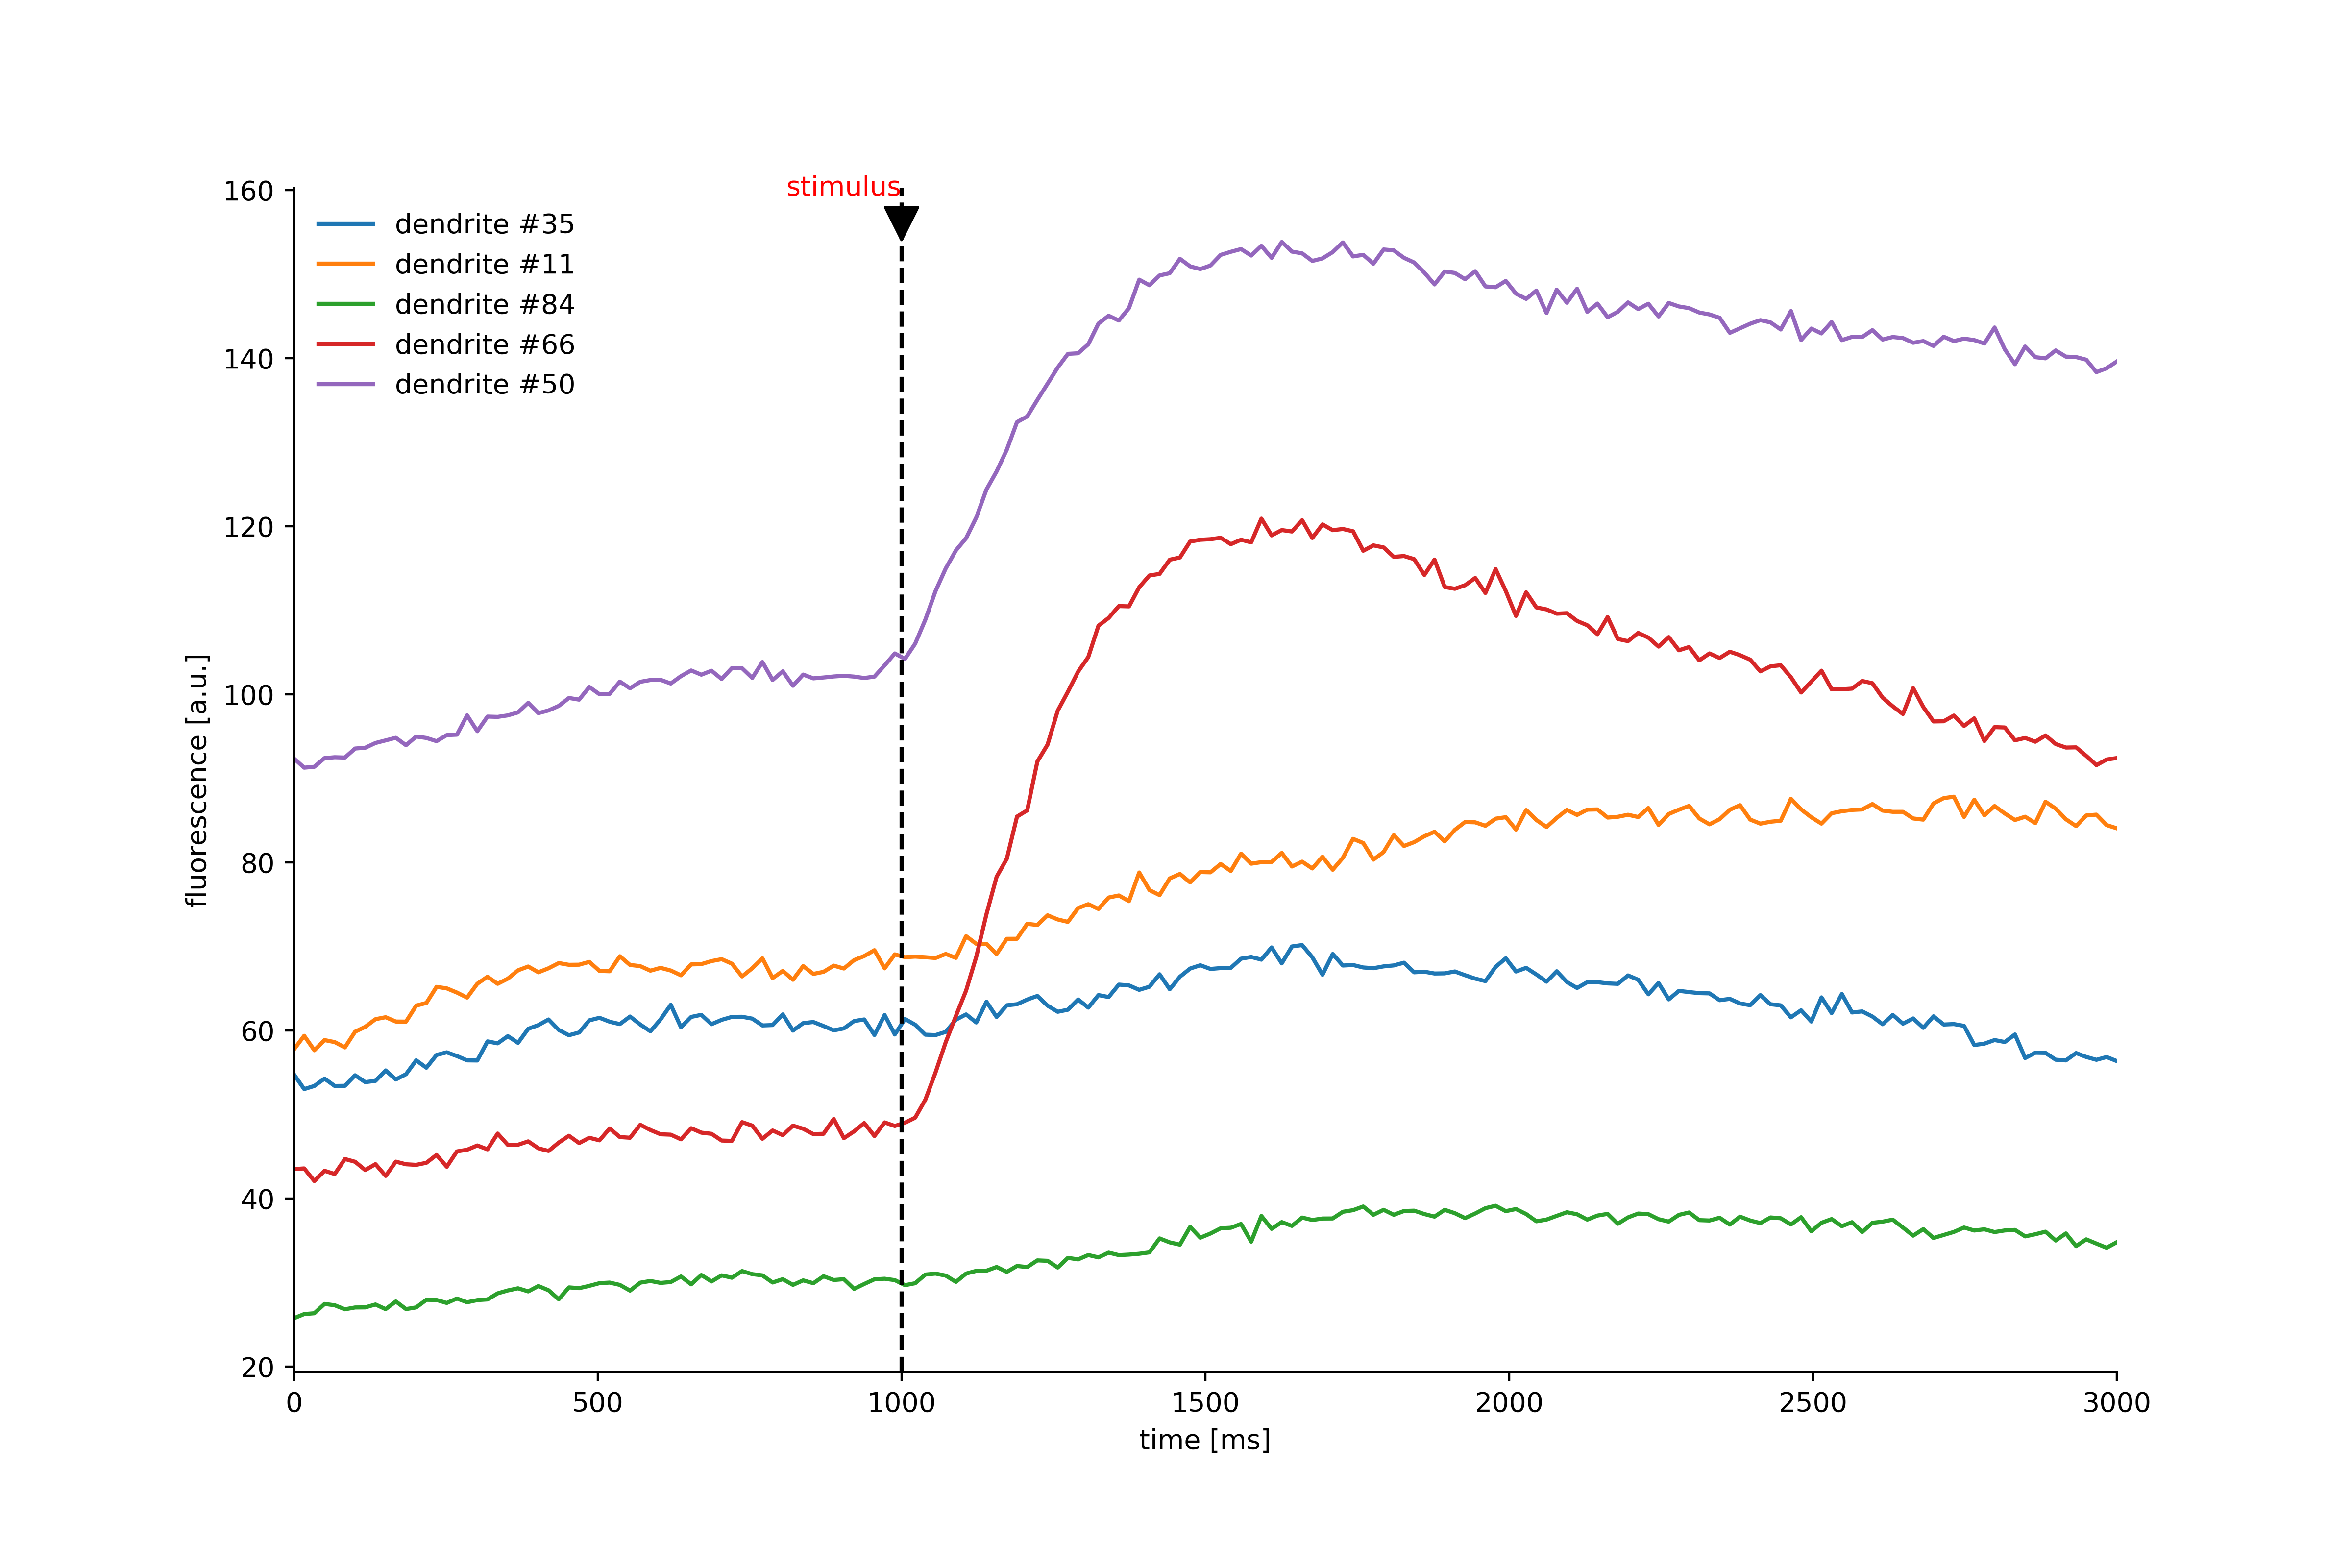
\includegraphics[scale=0.35]{traces.png}
	\end{figure}
	\end{center}
\end{frame}

\begin{frame}[fragile]{The Data - Behavioral}
	\begin{center}
	\begin{figure}
      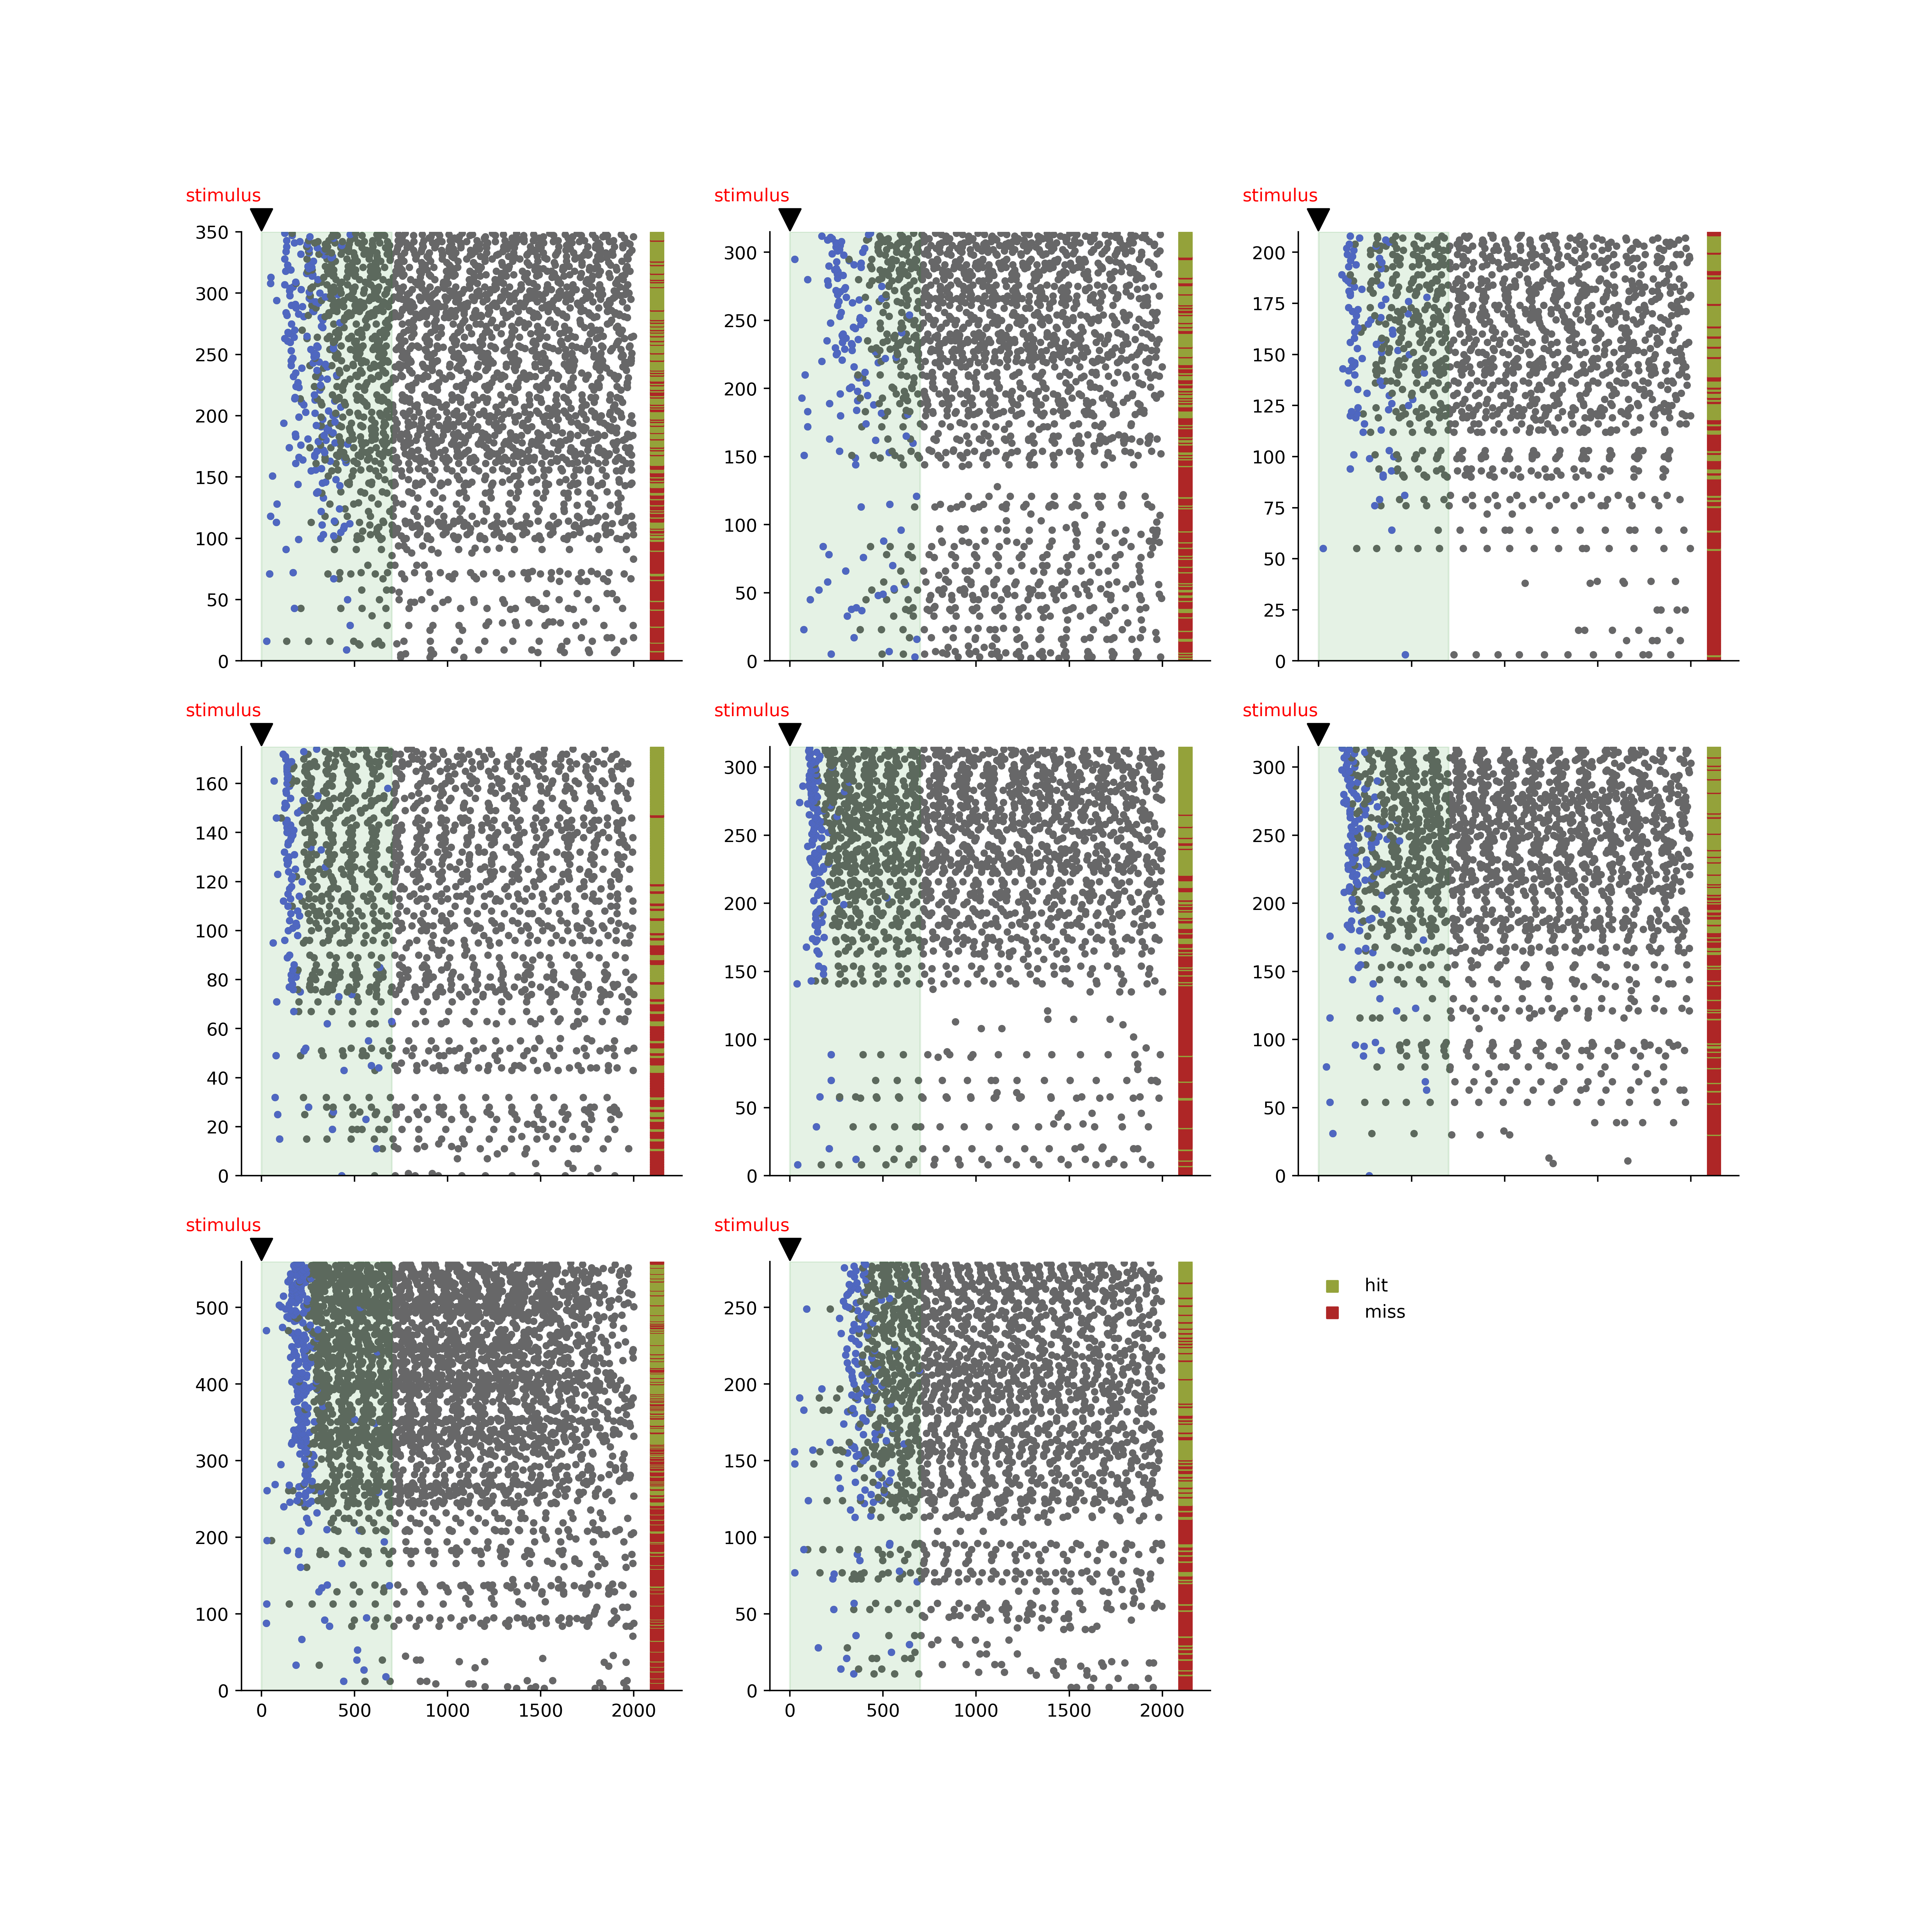
\includegraphics[scale=0.23	]{lickplots.png}
	\end{figure}
	\end{center}
\end{frame}

\begin{frame}[fragile]{The Data - Psychometric Curve}
\begin{center}
	\begin{figure}
      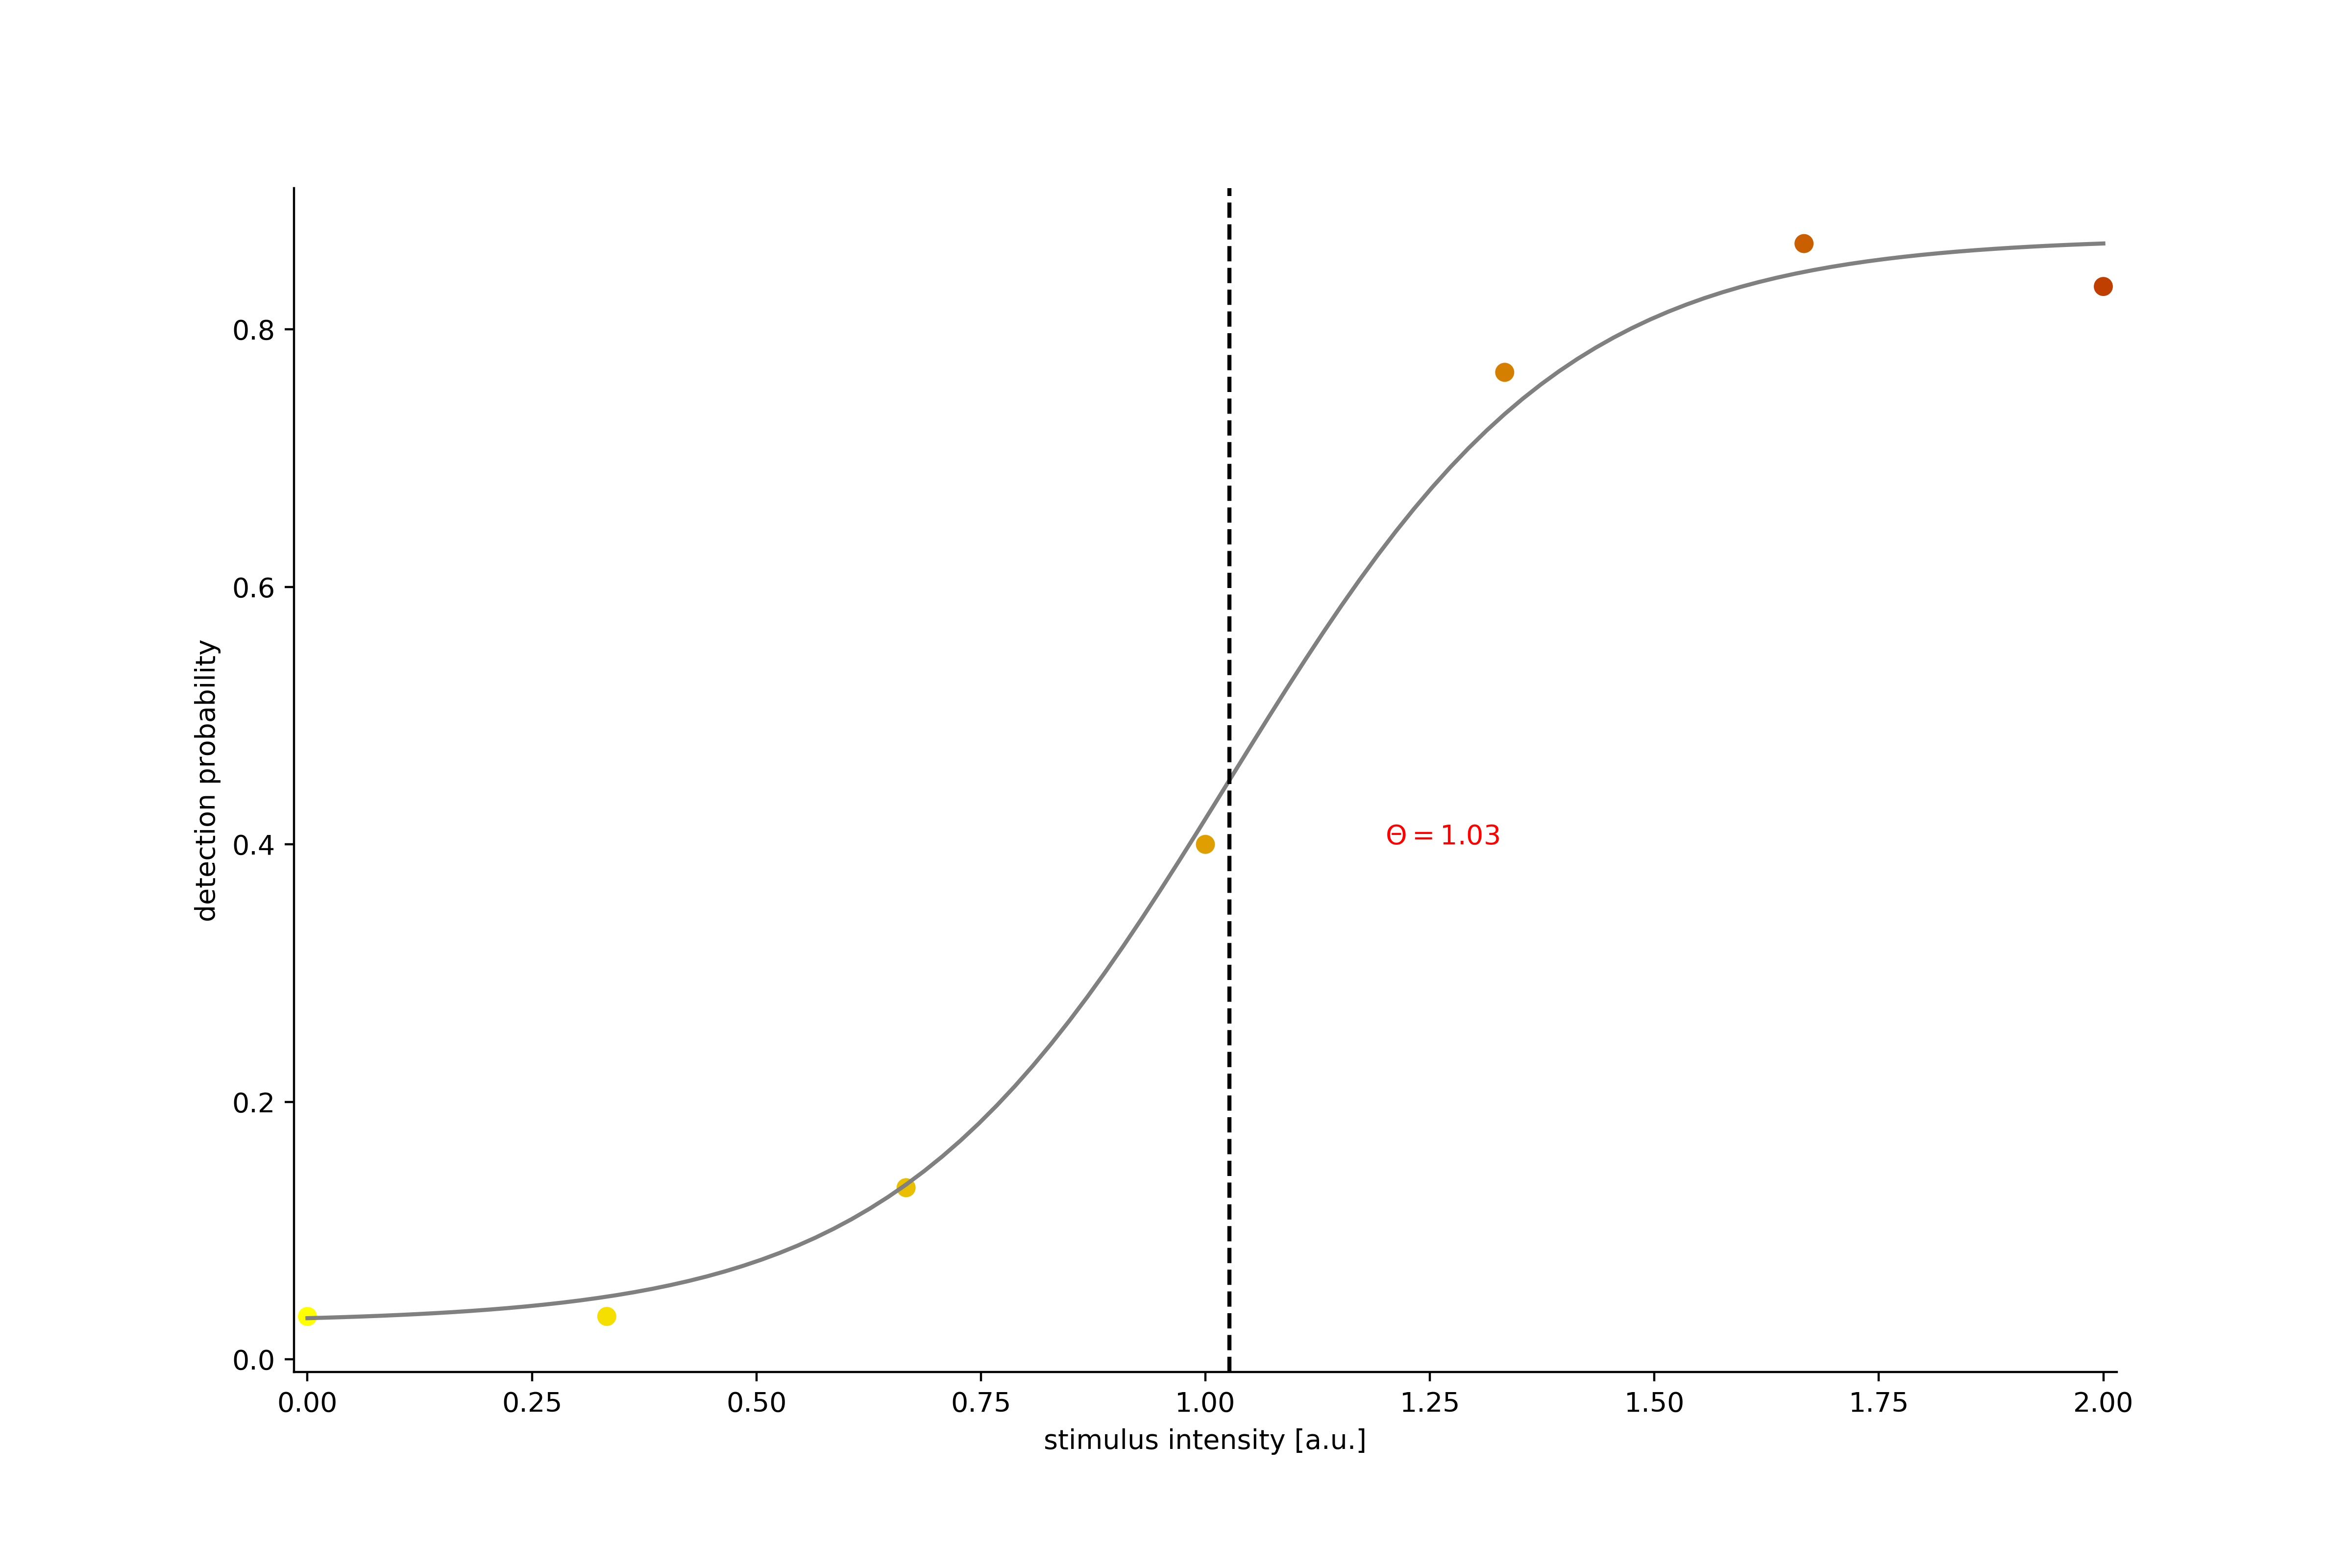
\includegraphics[scale=0.38]{psychometric.png}
	\end{figure}
	\end{center}
	
\end{frame}

\section{Goal}
\begin{frame}[fragile]{Goal}
The goal of this project is to investigate the following:
\begin{itemize}
\only<+->{
\item What information can we extract from the data?}
\only<+->{
\item What can we gain by doing multivariate analysis as opposed to univariate?}
\only<+->{
\item Can we say something about population coding?}
\end{itemize}
\end{frame}

\section{Univariate Analysis}

\begin{frame}[fragile]{Stimulus Presence Detection}
\begin{itemize}
\item Feature: mean activity of dendrite over one second after stimulus
\item Class one: all trials with stimulus strength 0
\item Class two: all trials with selected stimulus strength $(\neq 0)$
\end{itemize}
\end{frame}

\begin{frame}[fragile]{ROC}
\begin{center}
	\begin{figure}
      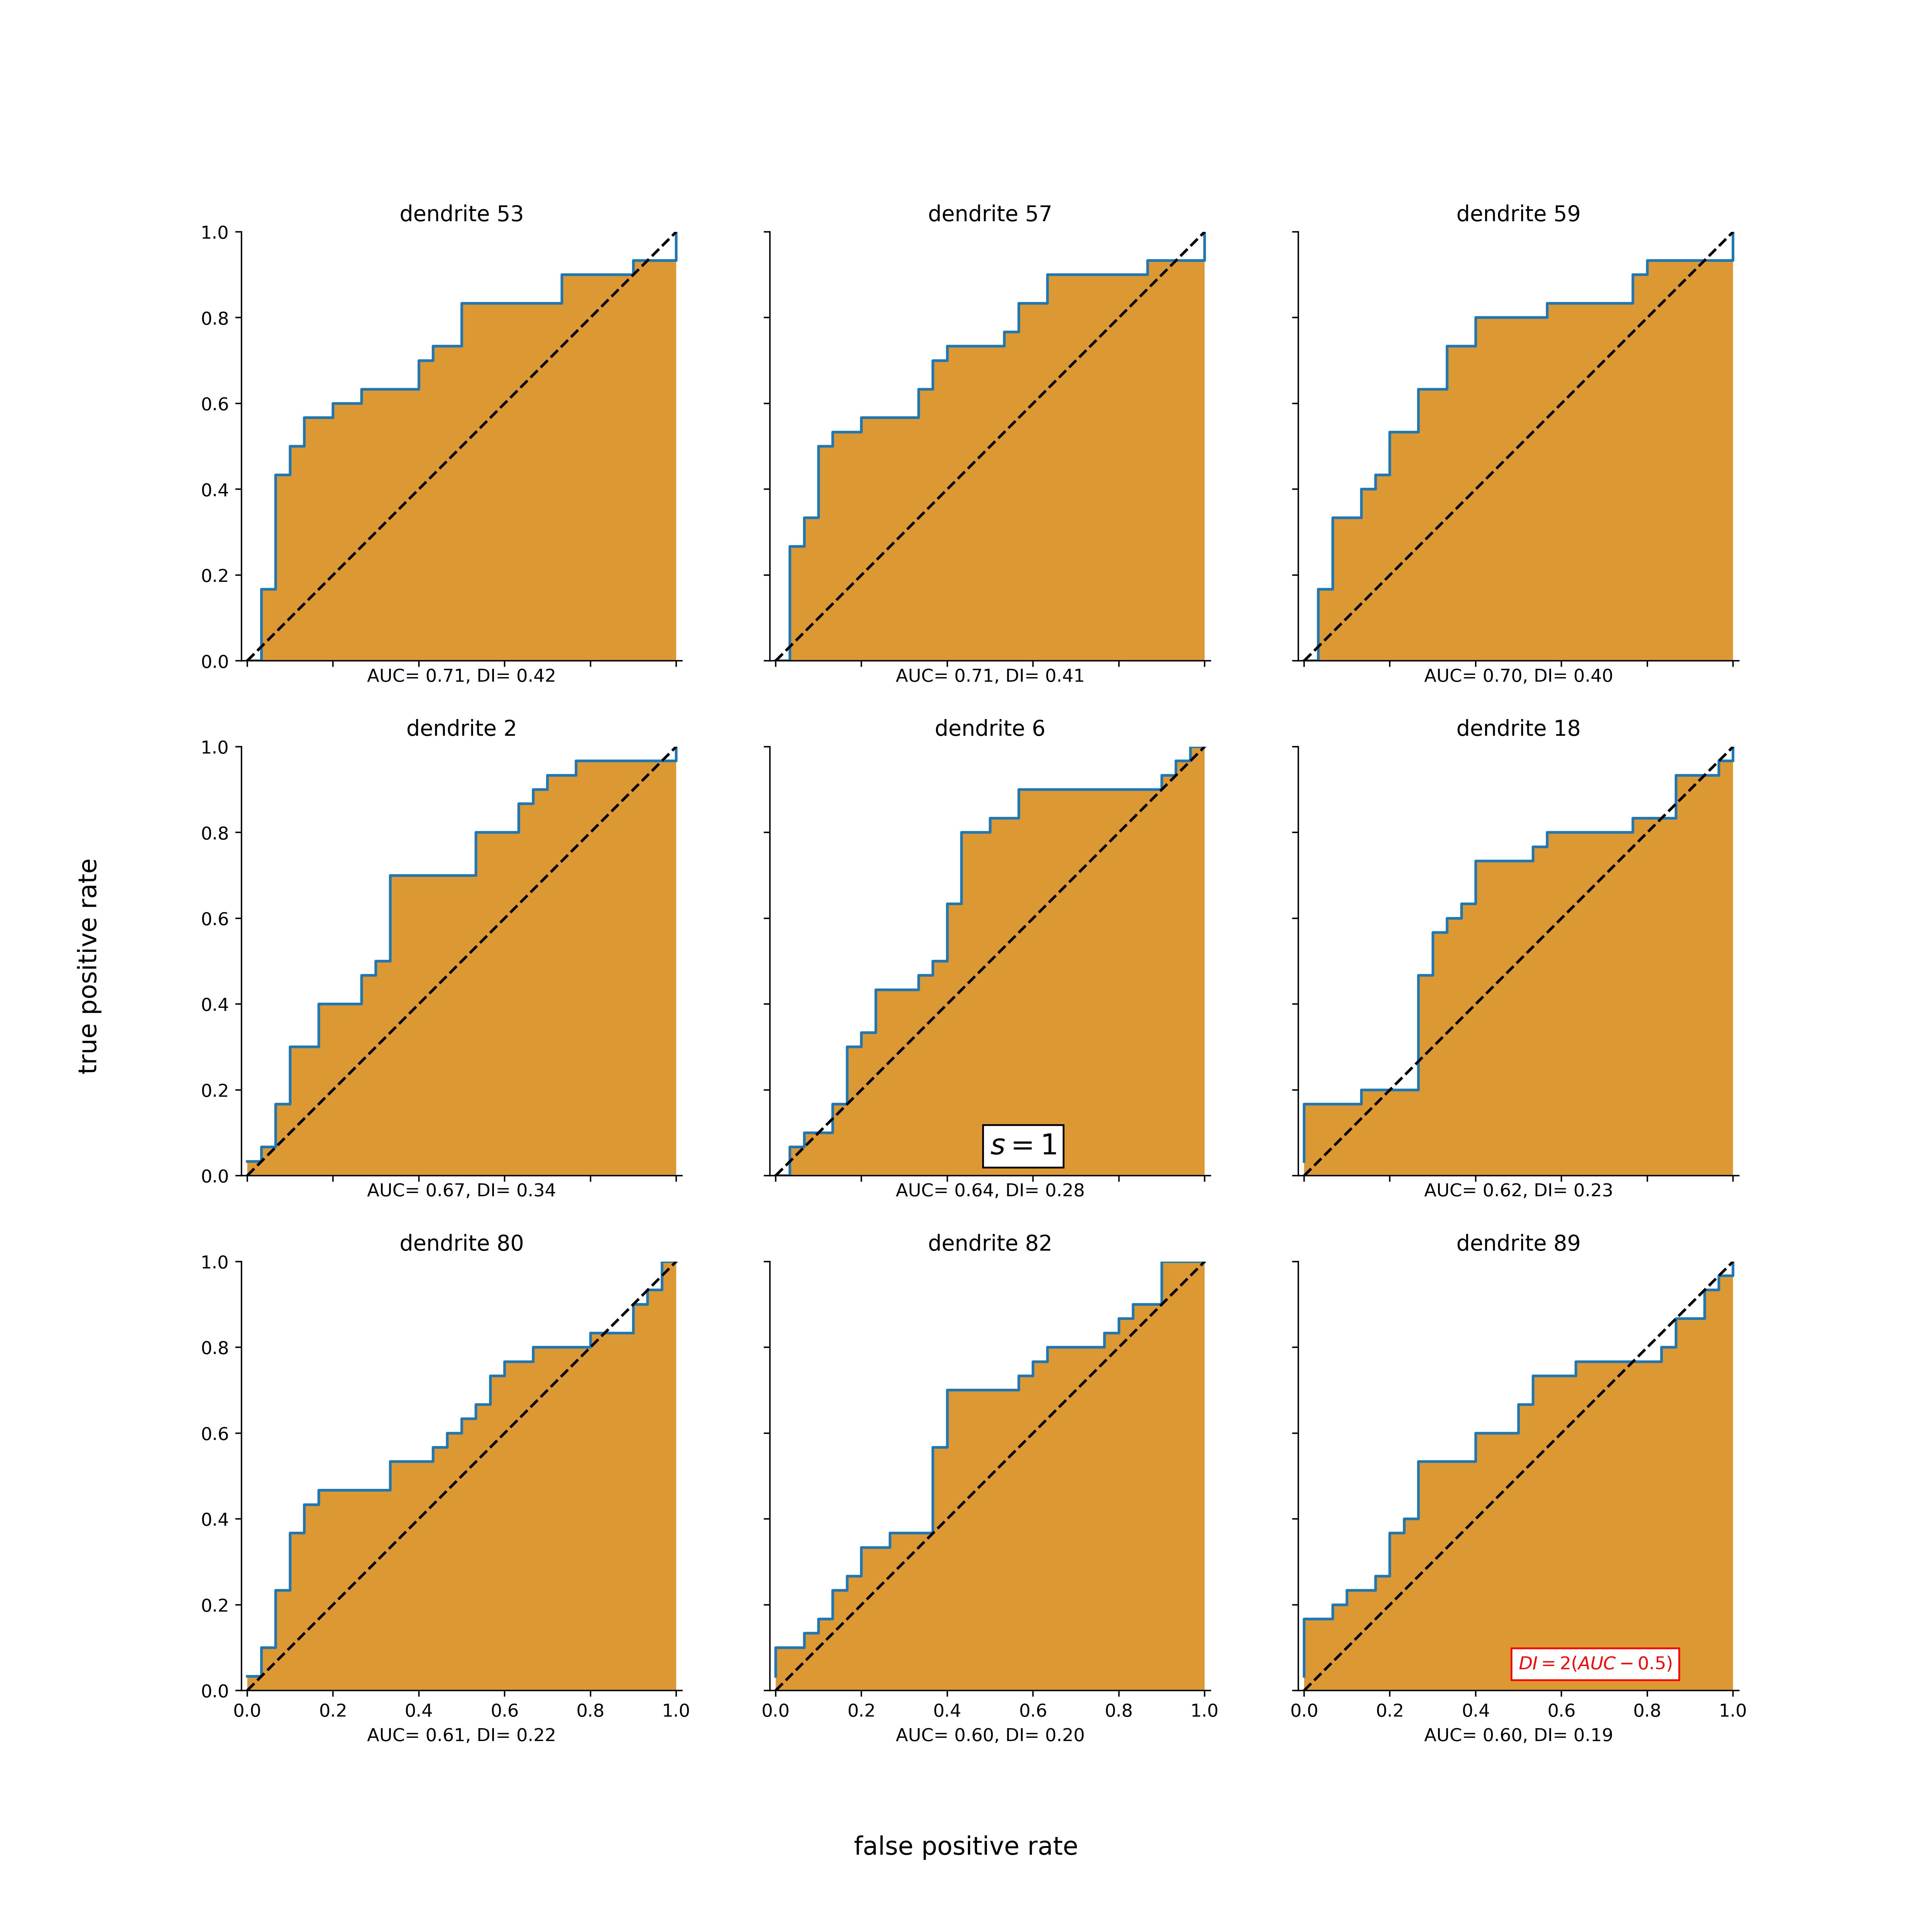
\includegraphics[width=0.75\textwidth]{roc_max.png}
	\end{figure}
	\end{center}
\end{frame}

%\begin{frame}[fragile]{Distribution of DI-Values}
%\begin{center}
%	\begin{figure}
%      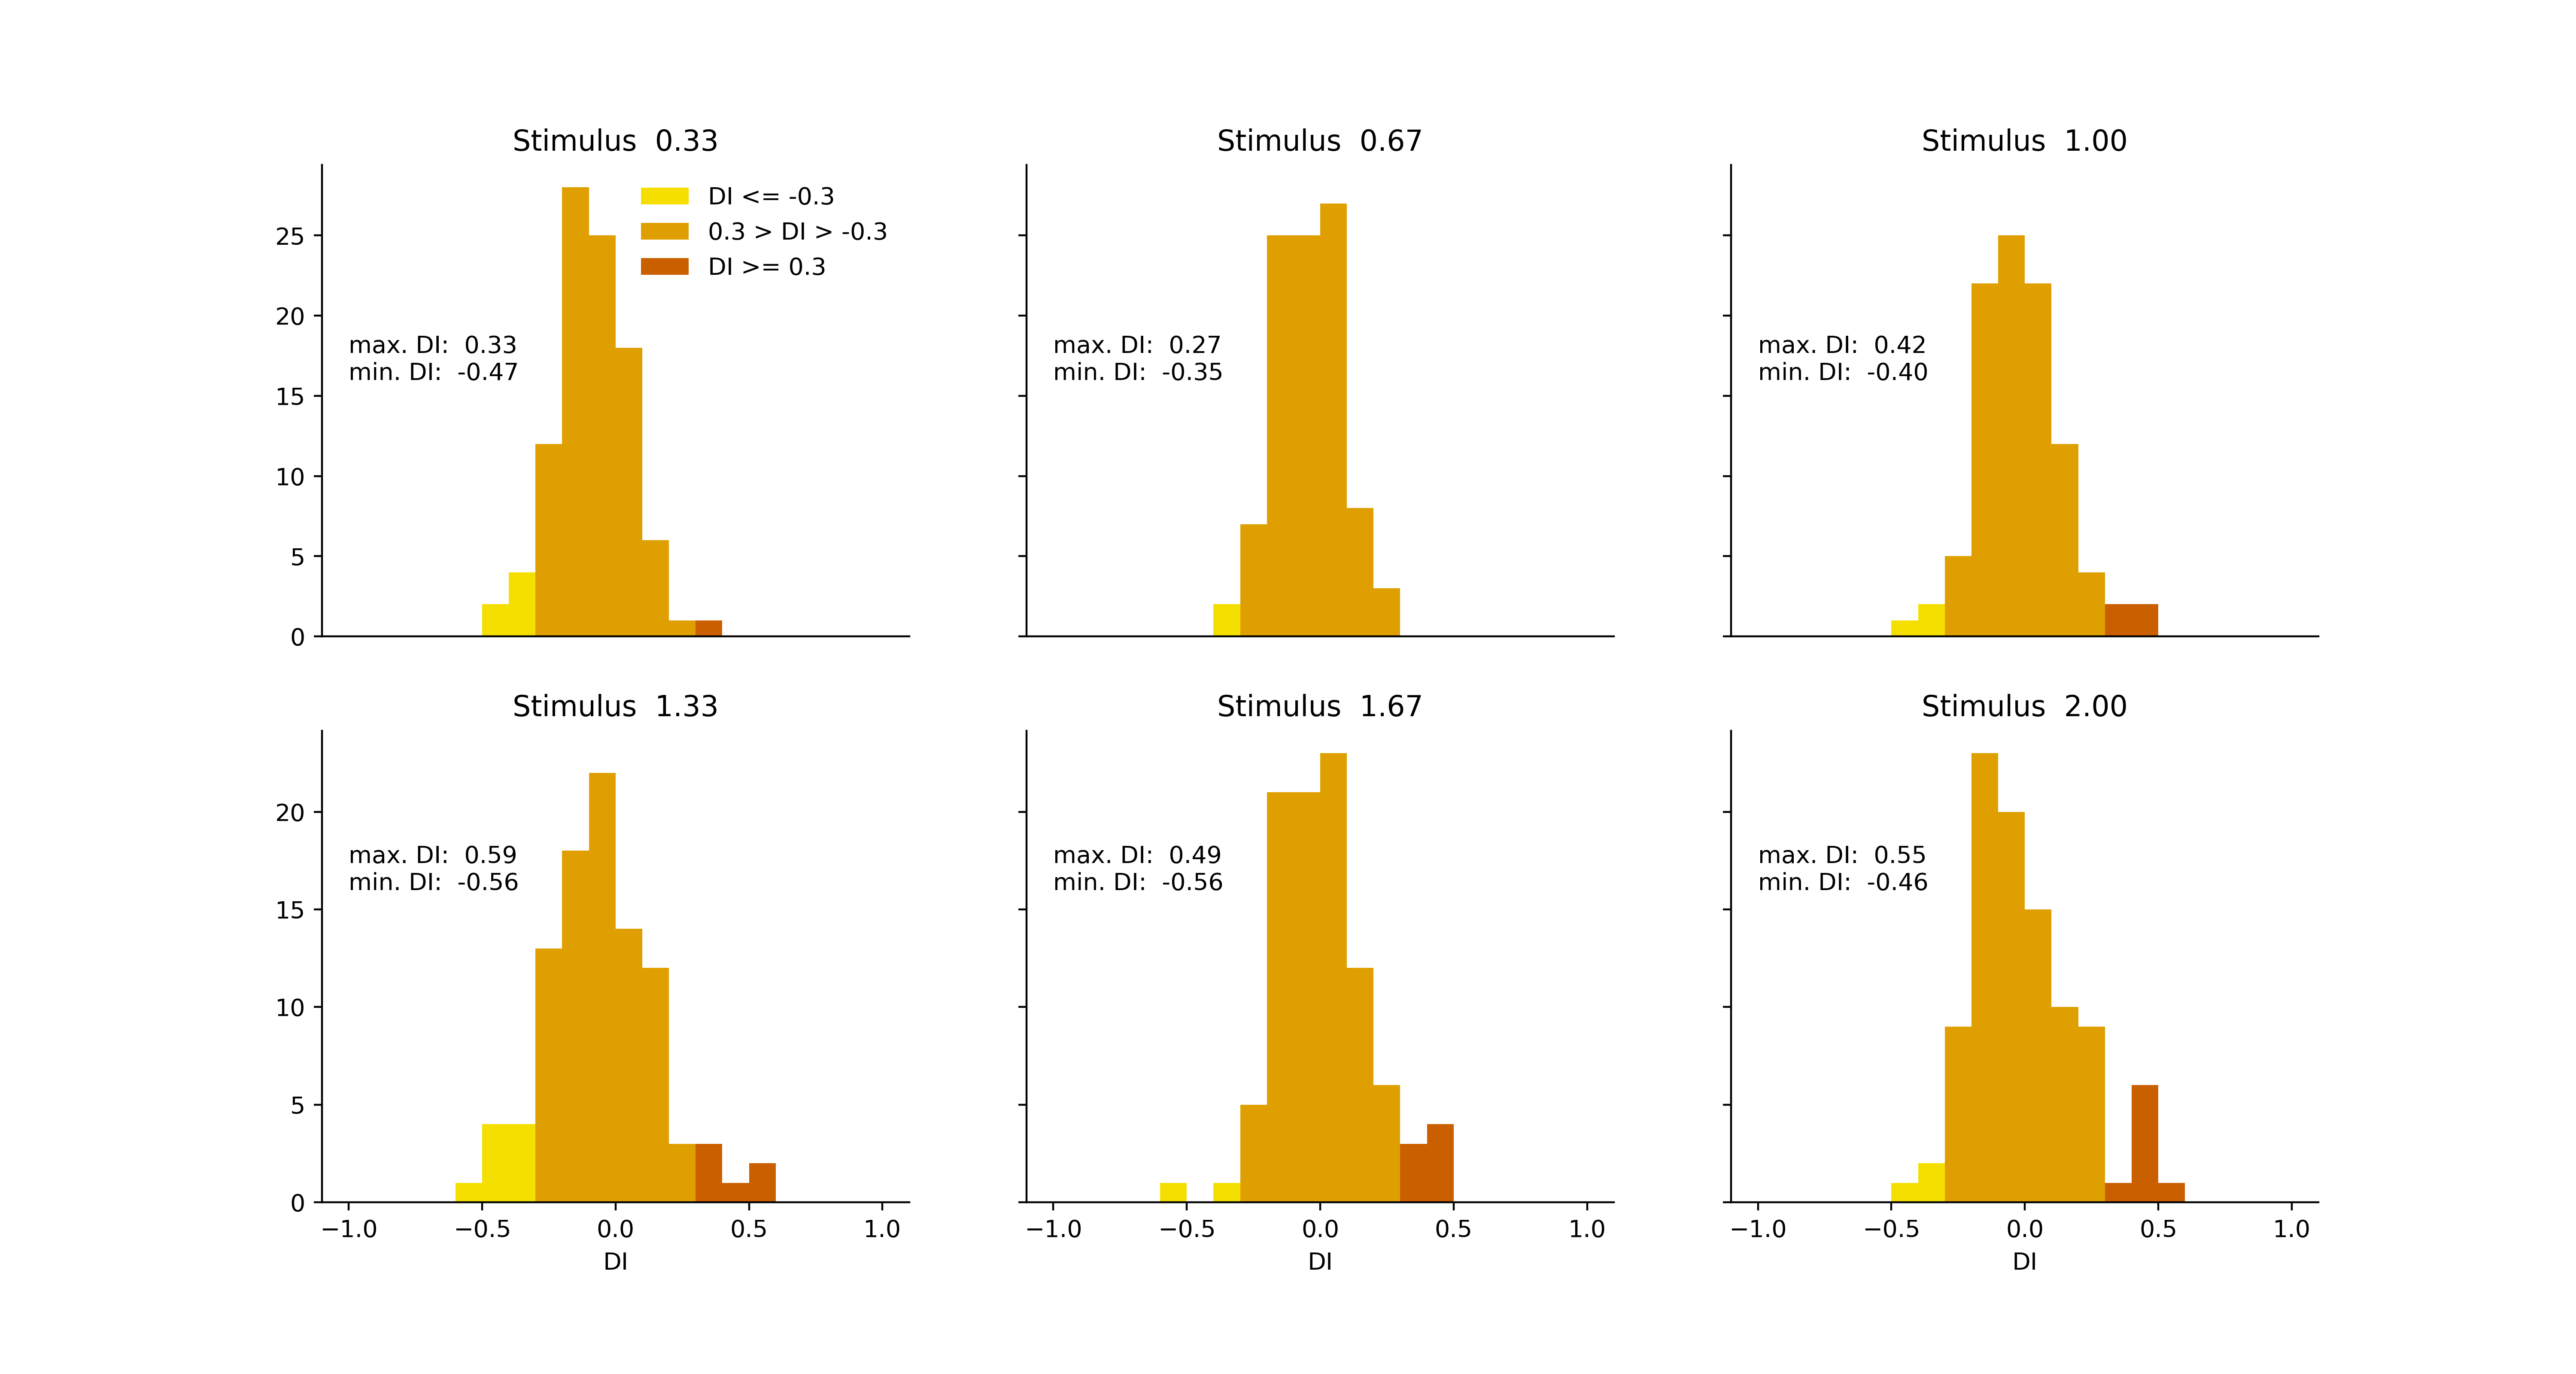
\includegraphics[width=1.0\textwidth]{DI_hist.png}
%	\end{figure}
%	\end{center}
%\end{frame}
%
%\begin{frame}[fragile]{Distribution of DI-Values vs. Chance}
%\begin{center}
%	\begin{figure}
%      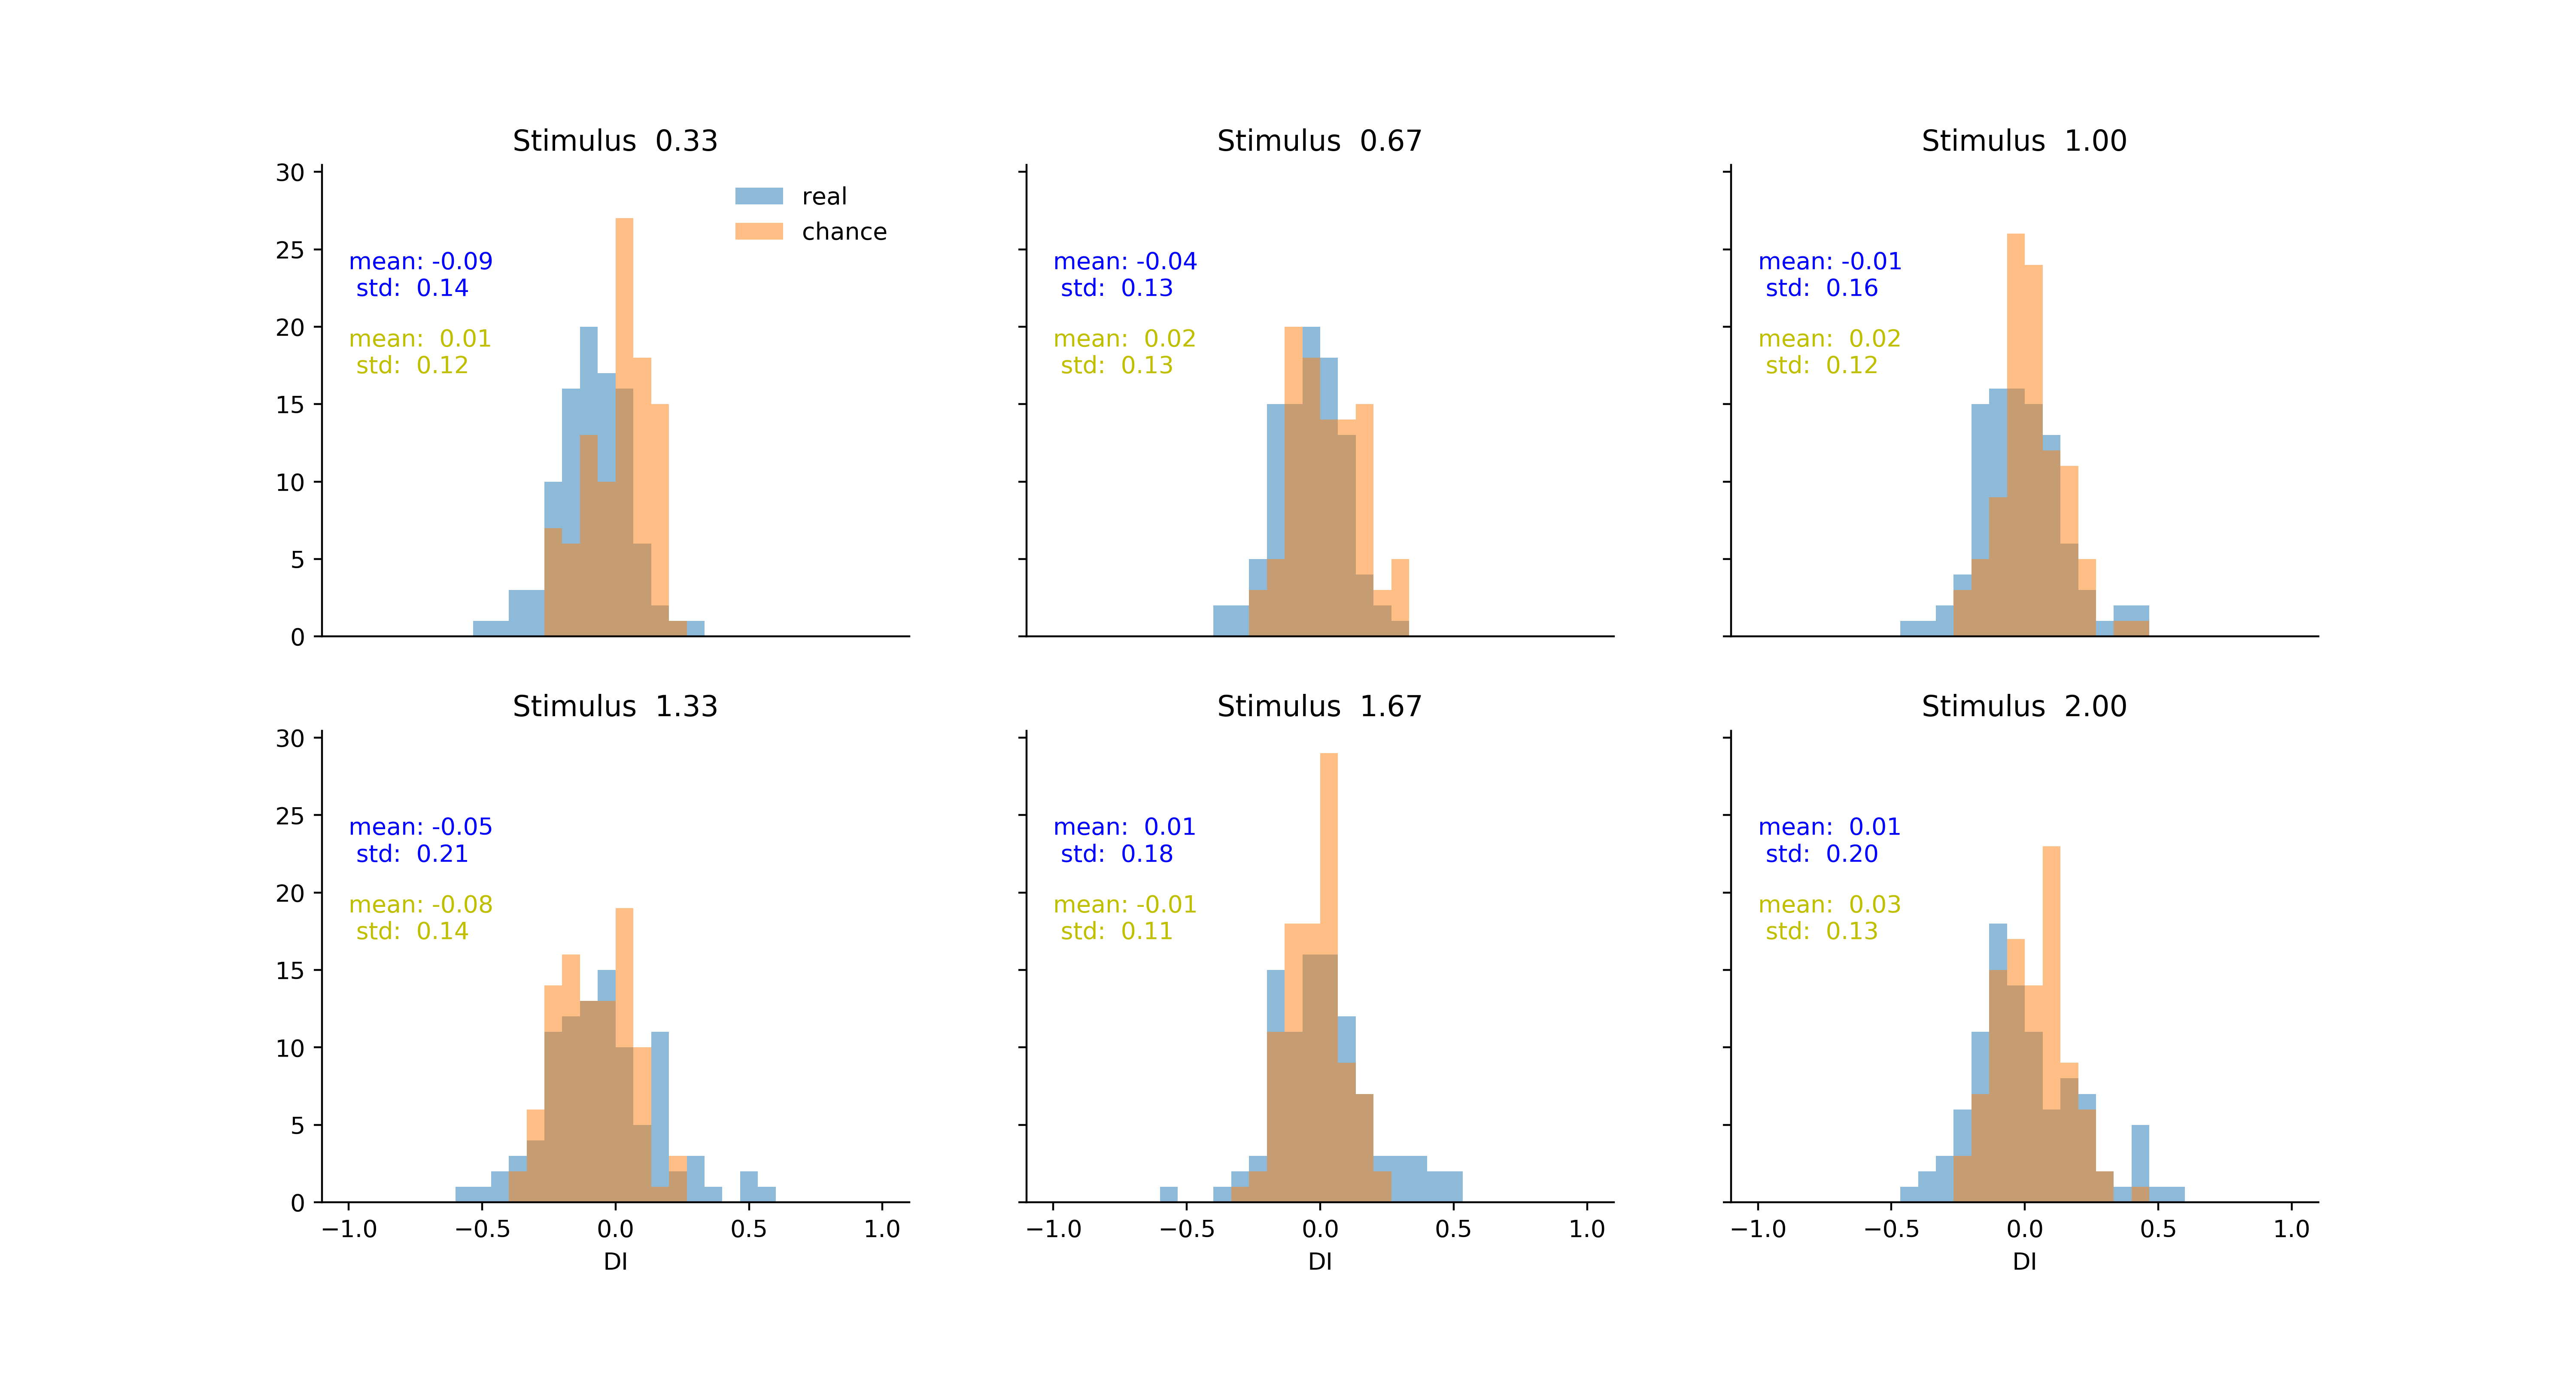
\includegraphics[width=1.0\textwidth]{realchance.png}
%	\end{figure}
%	\end{center}
%\end{frame}

\begin{frame}[fragile]{$\text{Ca}^{2+}$-Trace of Largest $|\text{DI}|$-Dendrites}
\begin{center}
	\begin{figure}
      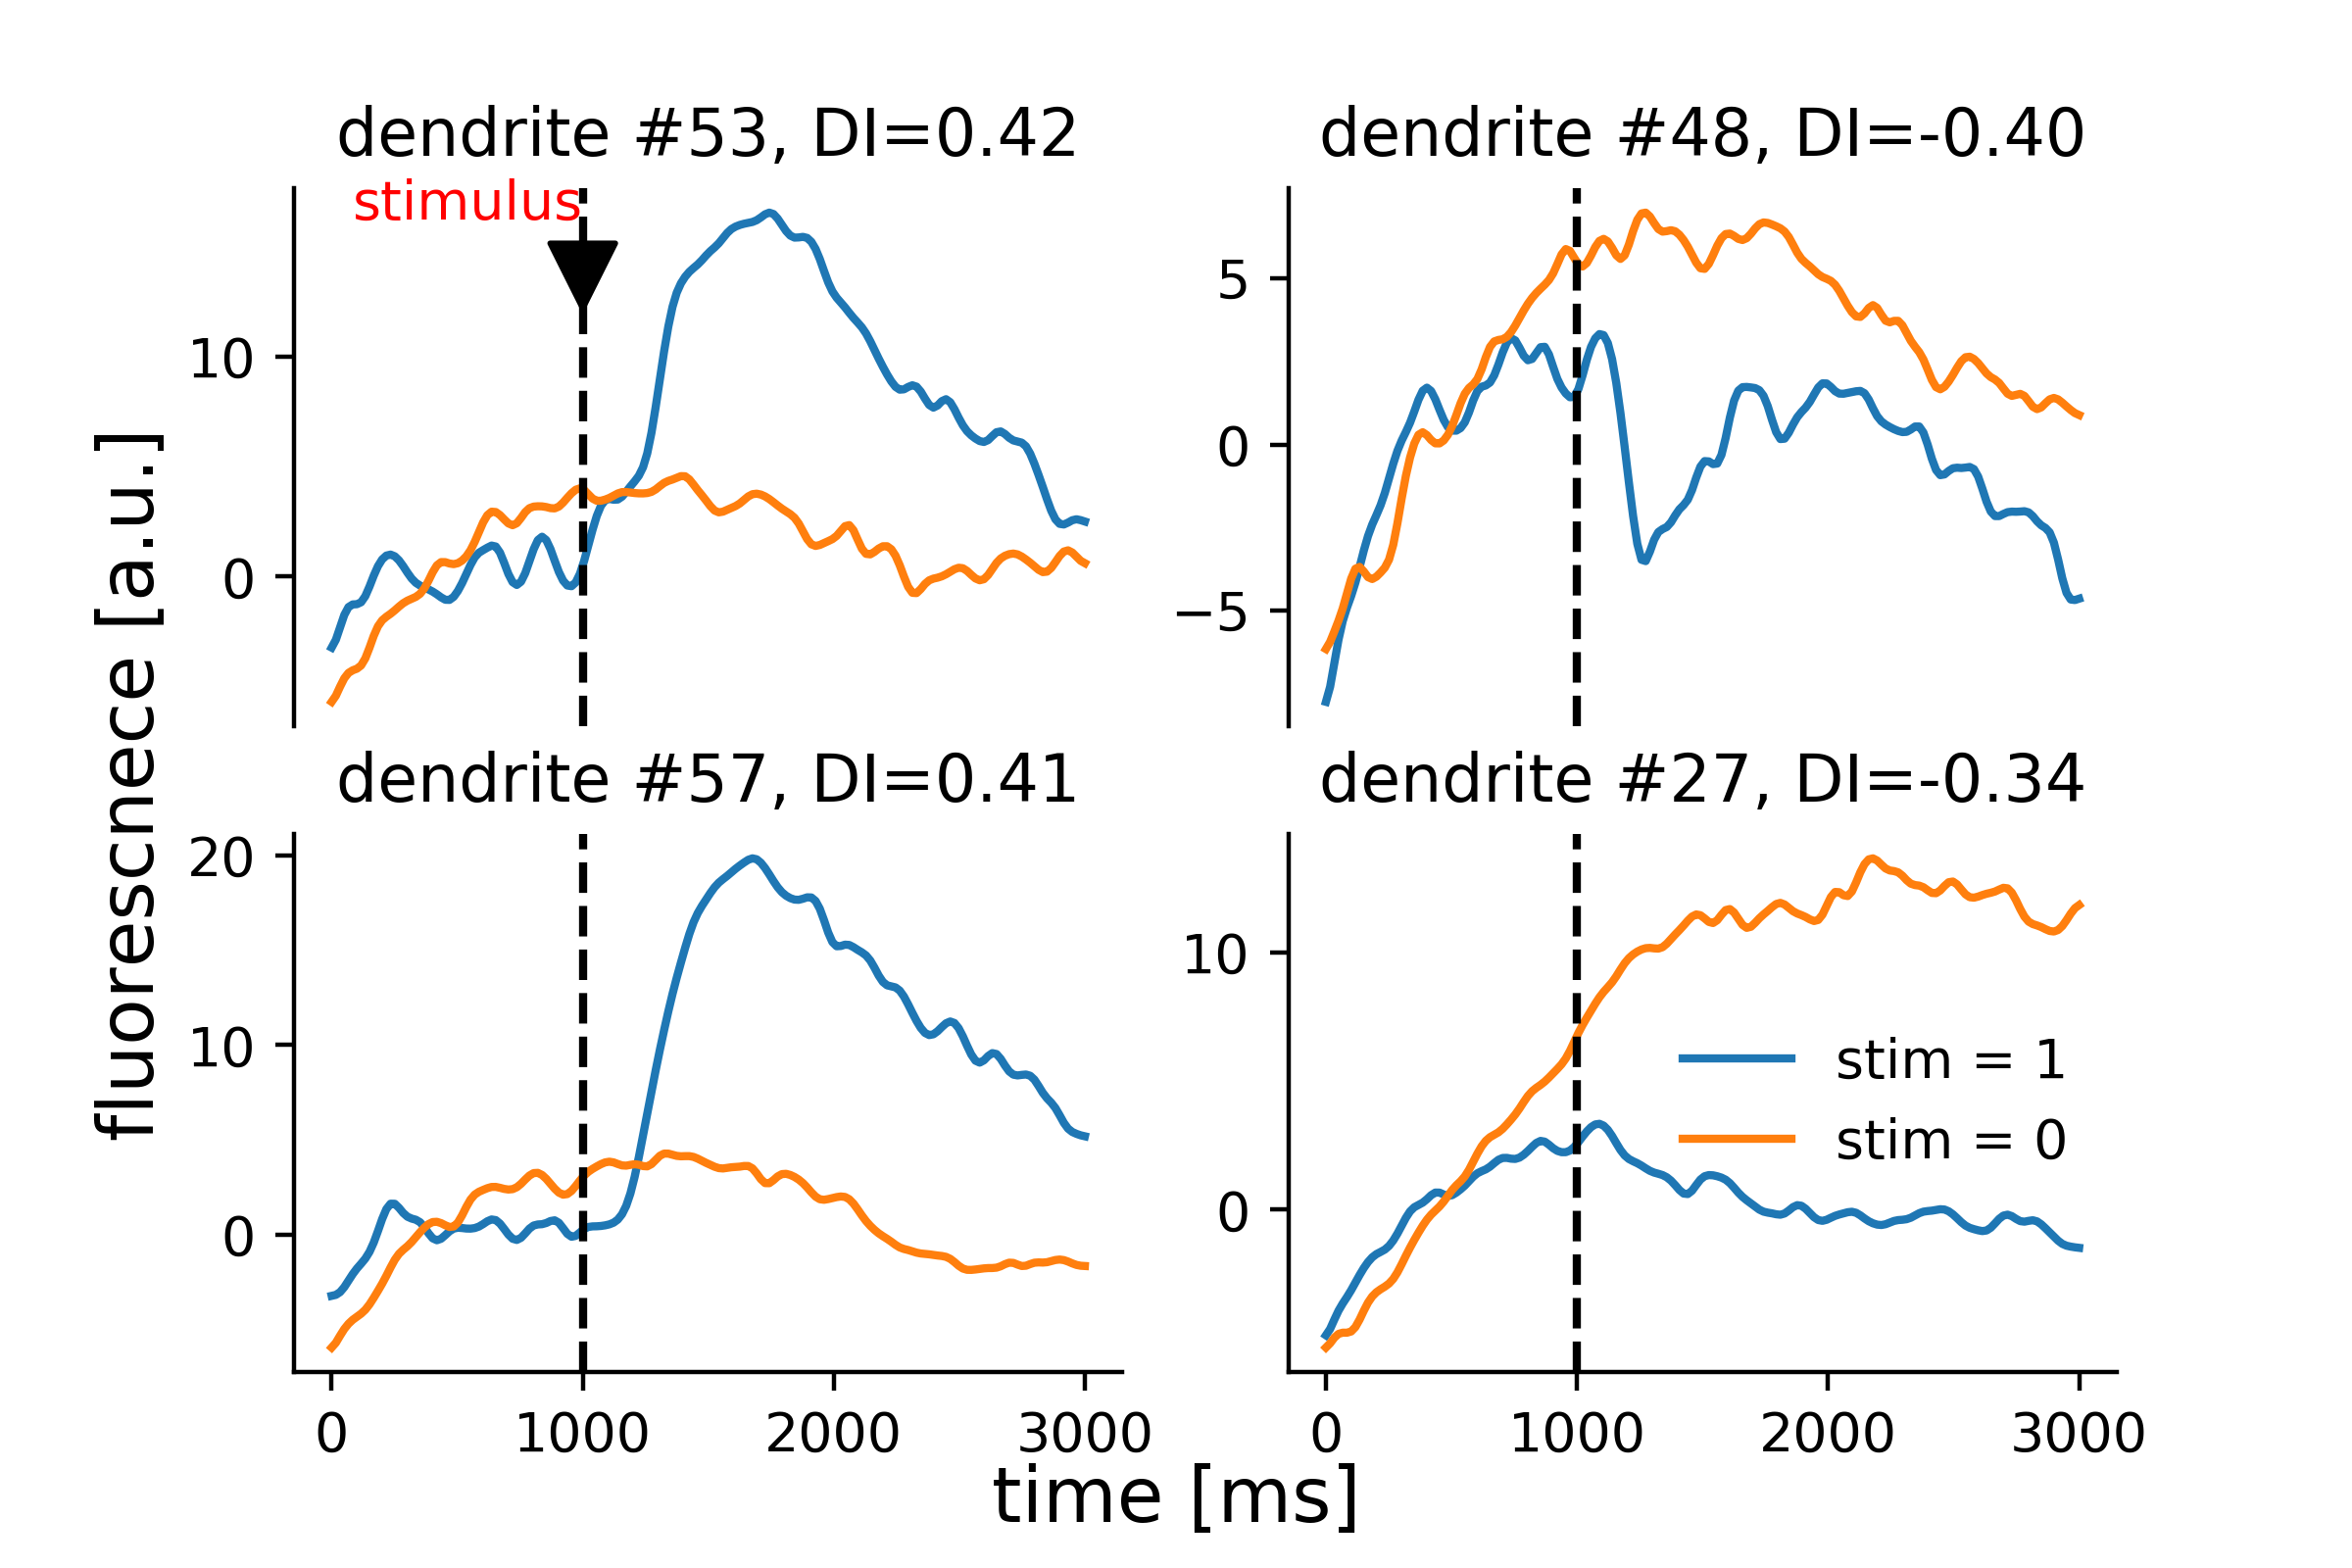
\includegraphics[width=1.0\textwidth]{on_vs_off.png}
      \caption*{Near threshold-stimulus ($\approx 1$)}
	\end{figure}
	\end{center}
\end{frame}

%\begin{frame}[fragile]{ROC Scores of Single Dendrites Using SVM}
%\begin{table}
%    \caption*{Stimulus strength 1 (near thereshold). Something is fishy here}
%    \begin{tabular}{c|c|c}
%      \toprule
%      Dendrite \# & Mean Accuracy & Standard Deviation\\
%      \midrule
%      57 & 0.44 & +/- 0.51\\
%      53 & 0.40 & +/- 0.28\\
%      48 & 0.38 & +/- 0.49\\
%      2 & 0.37 & +/- 0.74\\
%      \bottomrule
%    \end{tabular}
%  \end{table}
%\end{frame}

\begin{frame}[fragile]{SVM - Most Accurate Dendrites}
\begin{table}
    \caption*{Stimulus strength 1 (near thereshold)}
    \begin{tabular}{c|c|c}
      \toprule
      Dendrite \# & $\mu_{acc}$ & $\sigma_{acc}$\\
      \midrule
      57 & 0.70 & 0.12\\
      53 & 0.68 & 0.14\\
      48 & 0.63 & 0.13\\
      27 & 0.62 & 0.08\\
      \bottomrule
    \end{tabular}
  \end{table}
\end{frame}

\begin{frame}[fragile]{Rank Order Correlations of Dendrites Over Stimuli}
\begin{center}
	\begin{figure}\caption*{Weighted rank coefficient $\rho_{\omega}$ (todo: find more optimal weights)}
      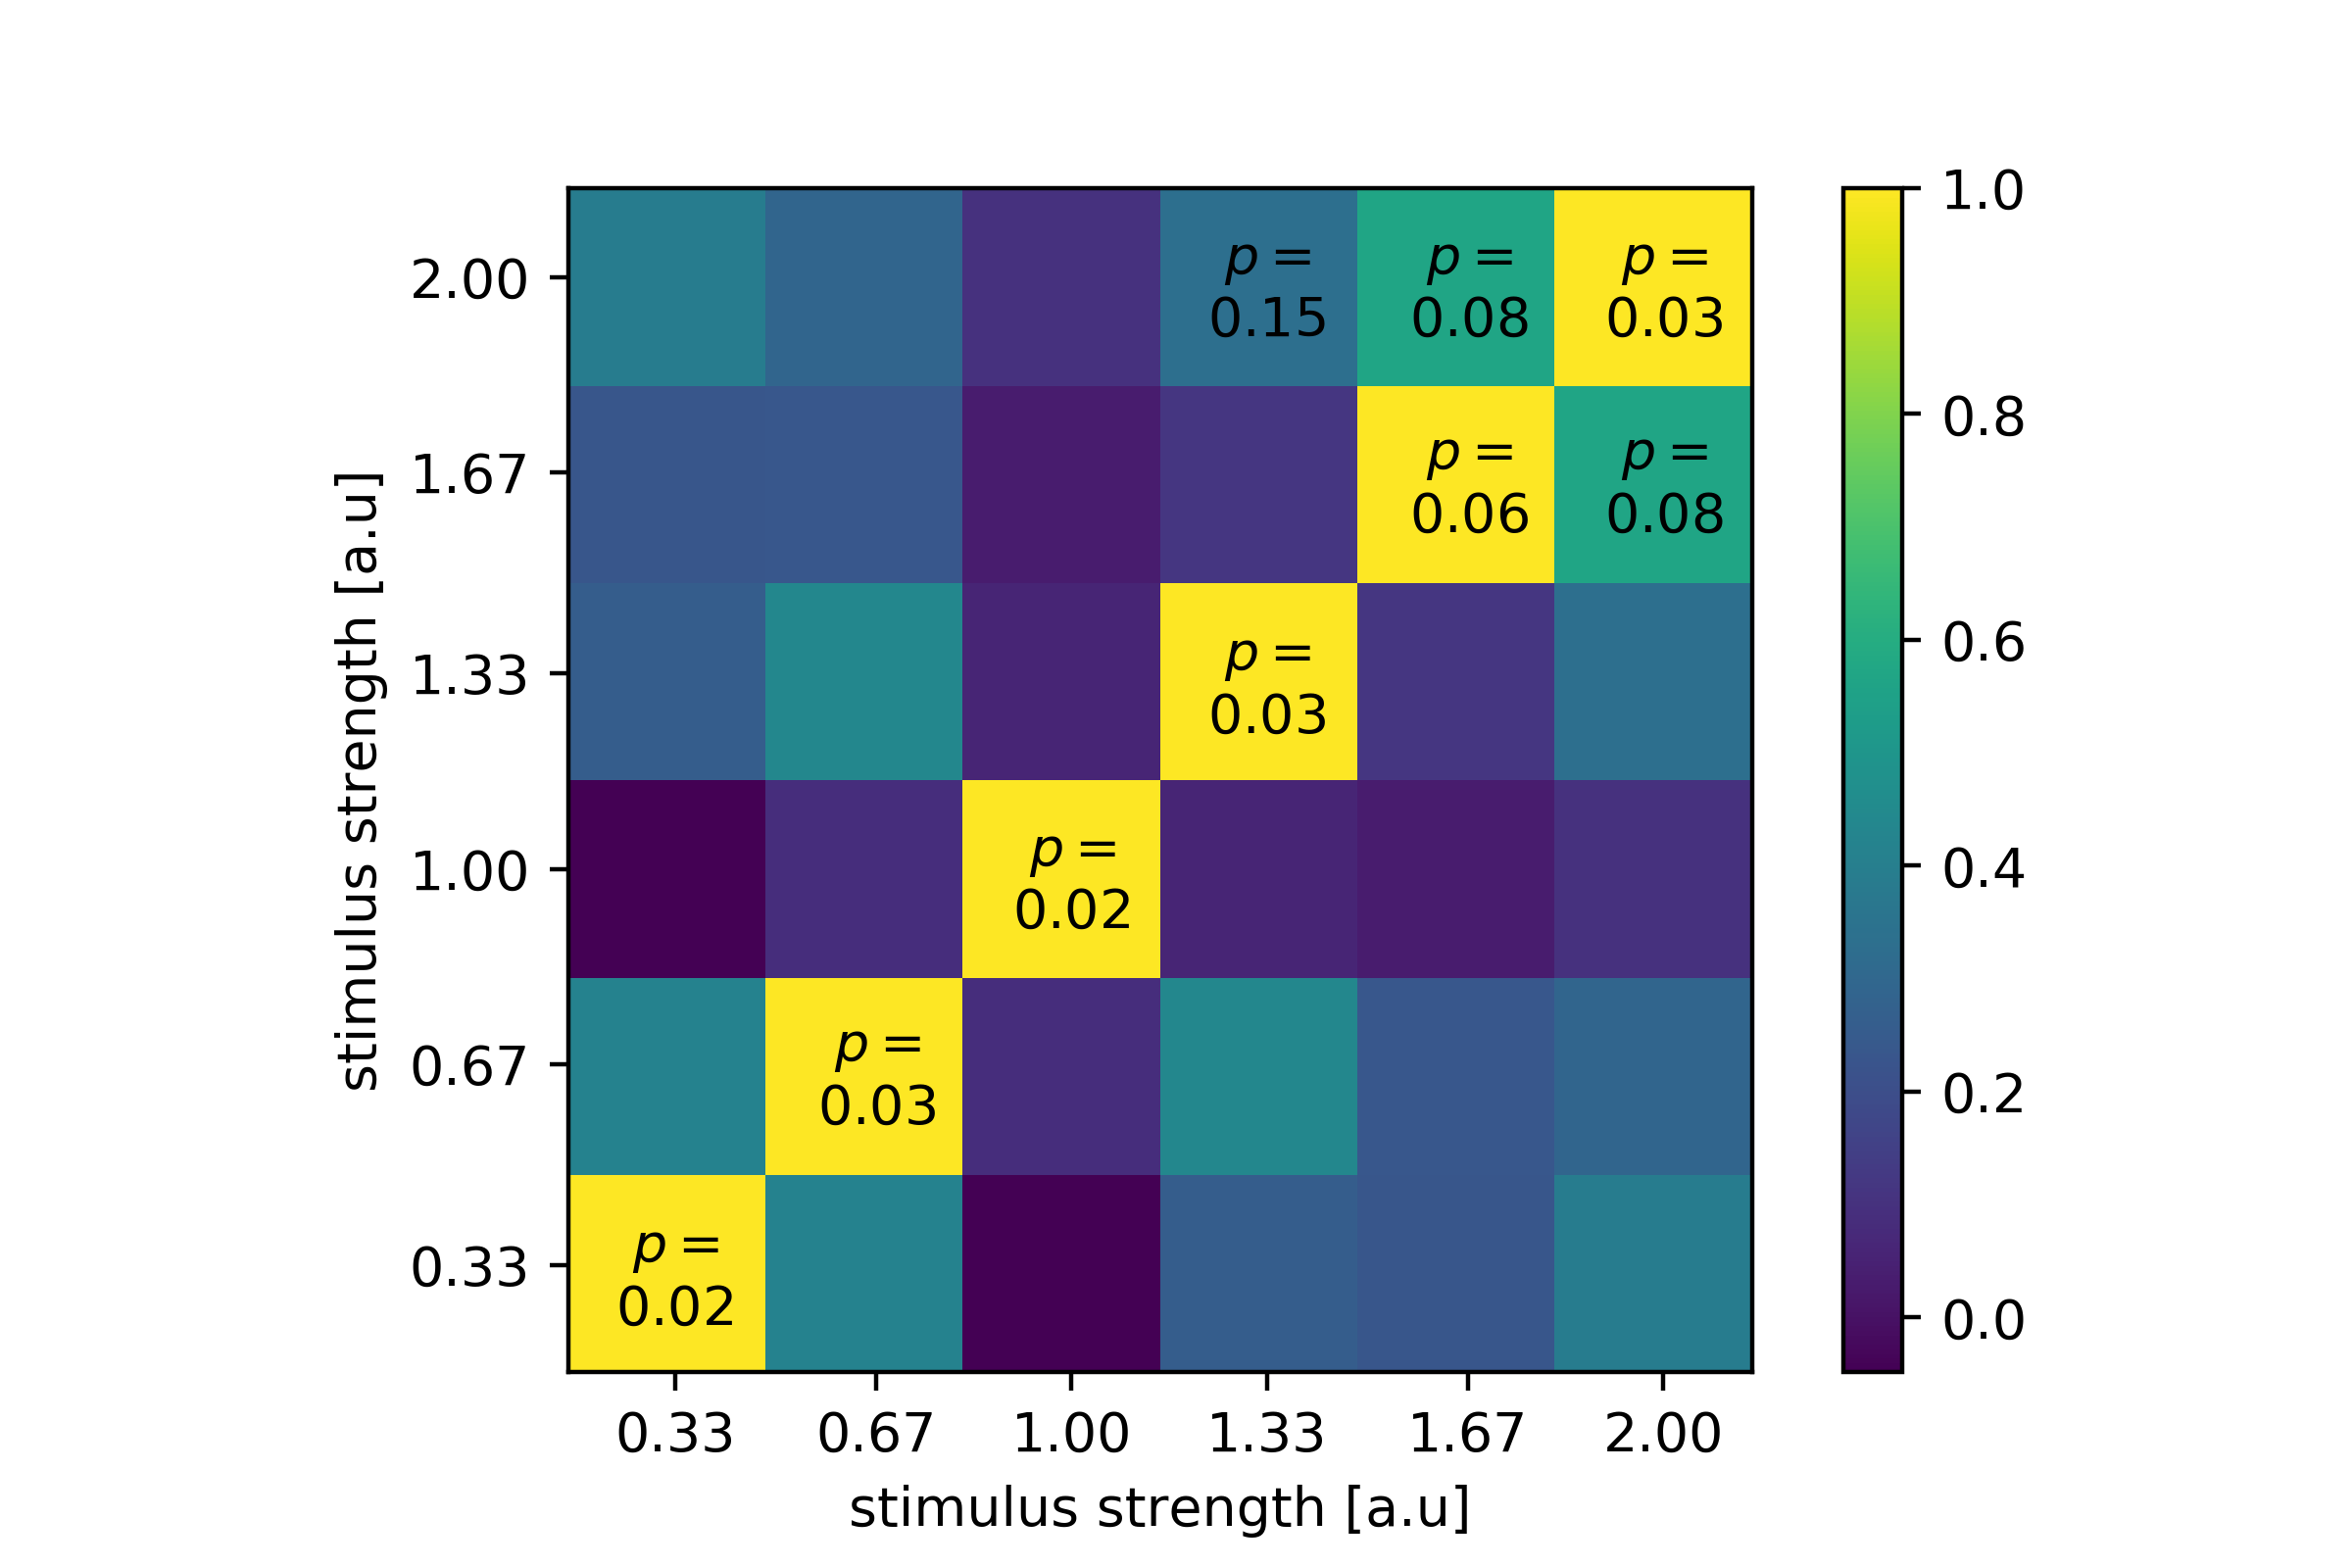
\includegraphics[width=1.0\textwidth]{rank_presence.png}
	\end{figure}
	\end{center}
\end{frame}

\begin{frame}[fragile]{DI and SVM Dendrtie Rank Order Correlation}
\begin{center}
	\begin{figure}
	\caption*{Something is wrong here, should be more correlation}
      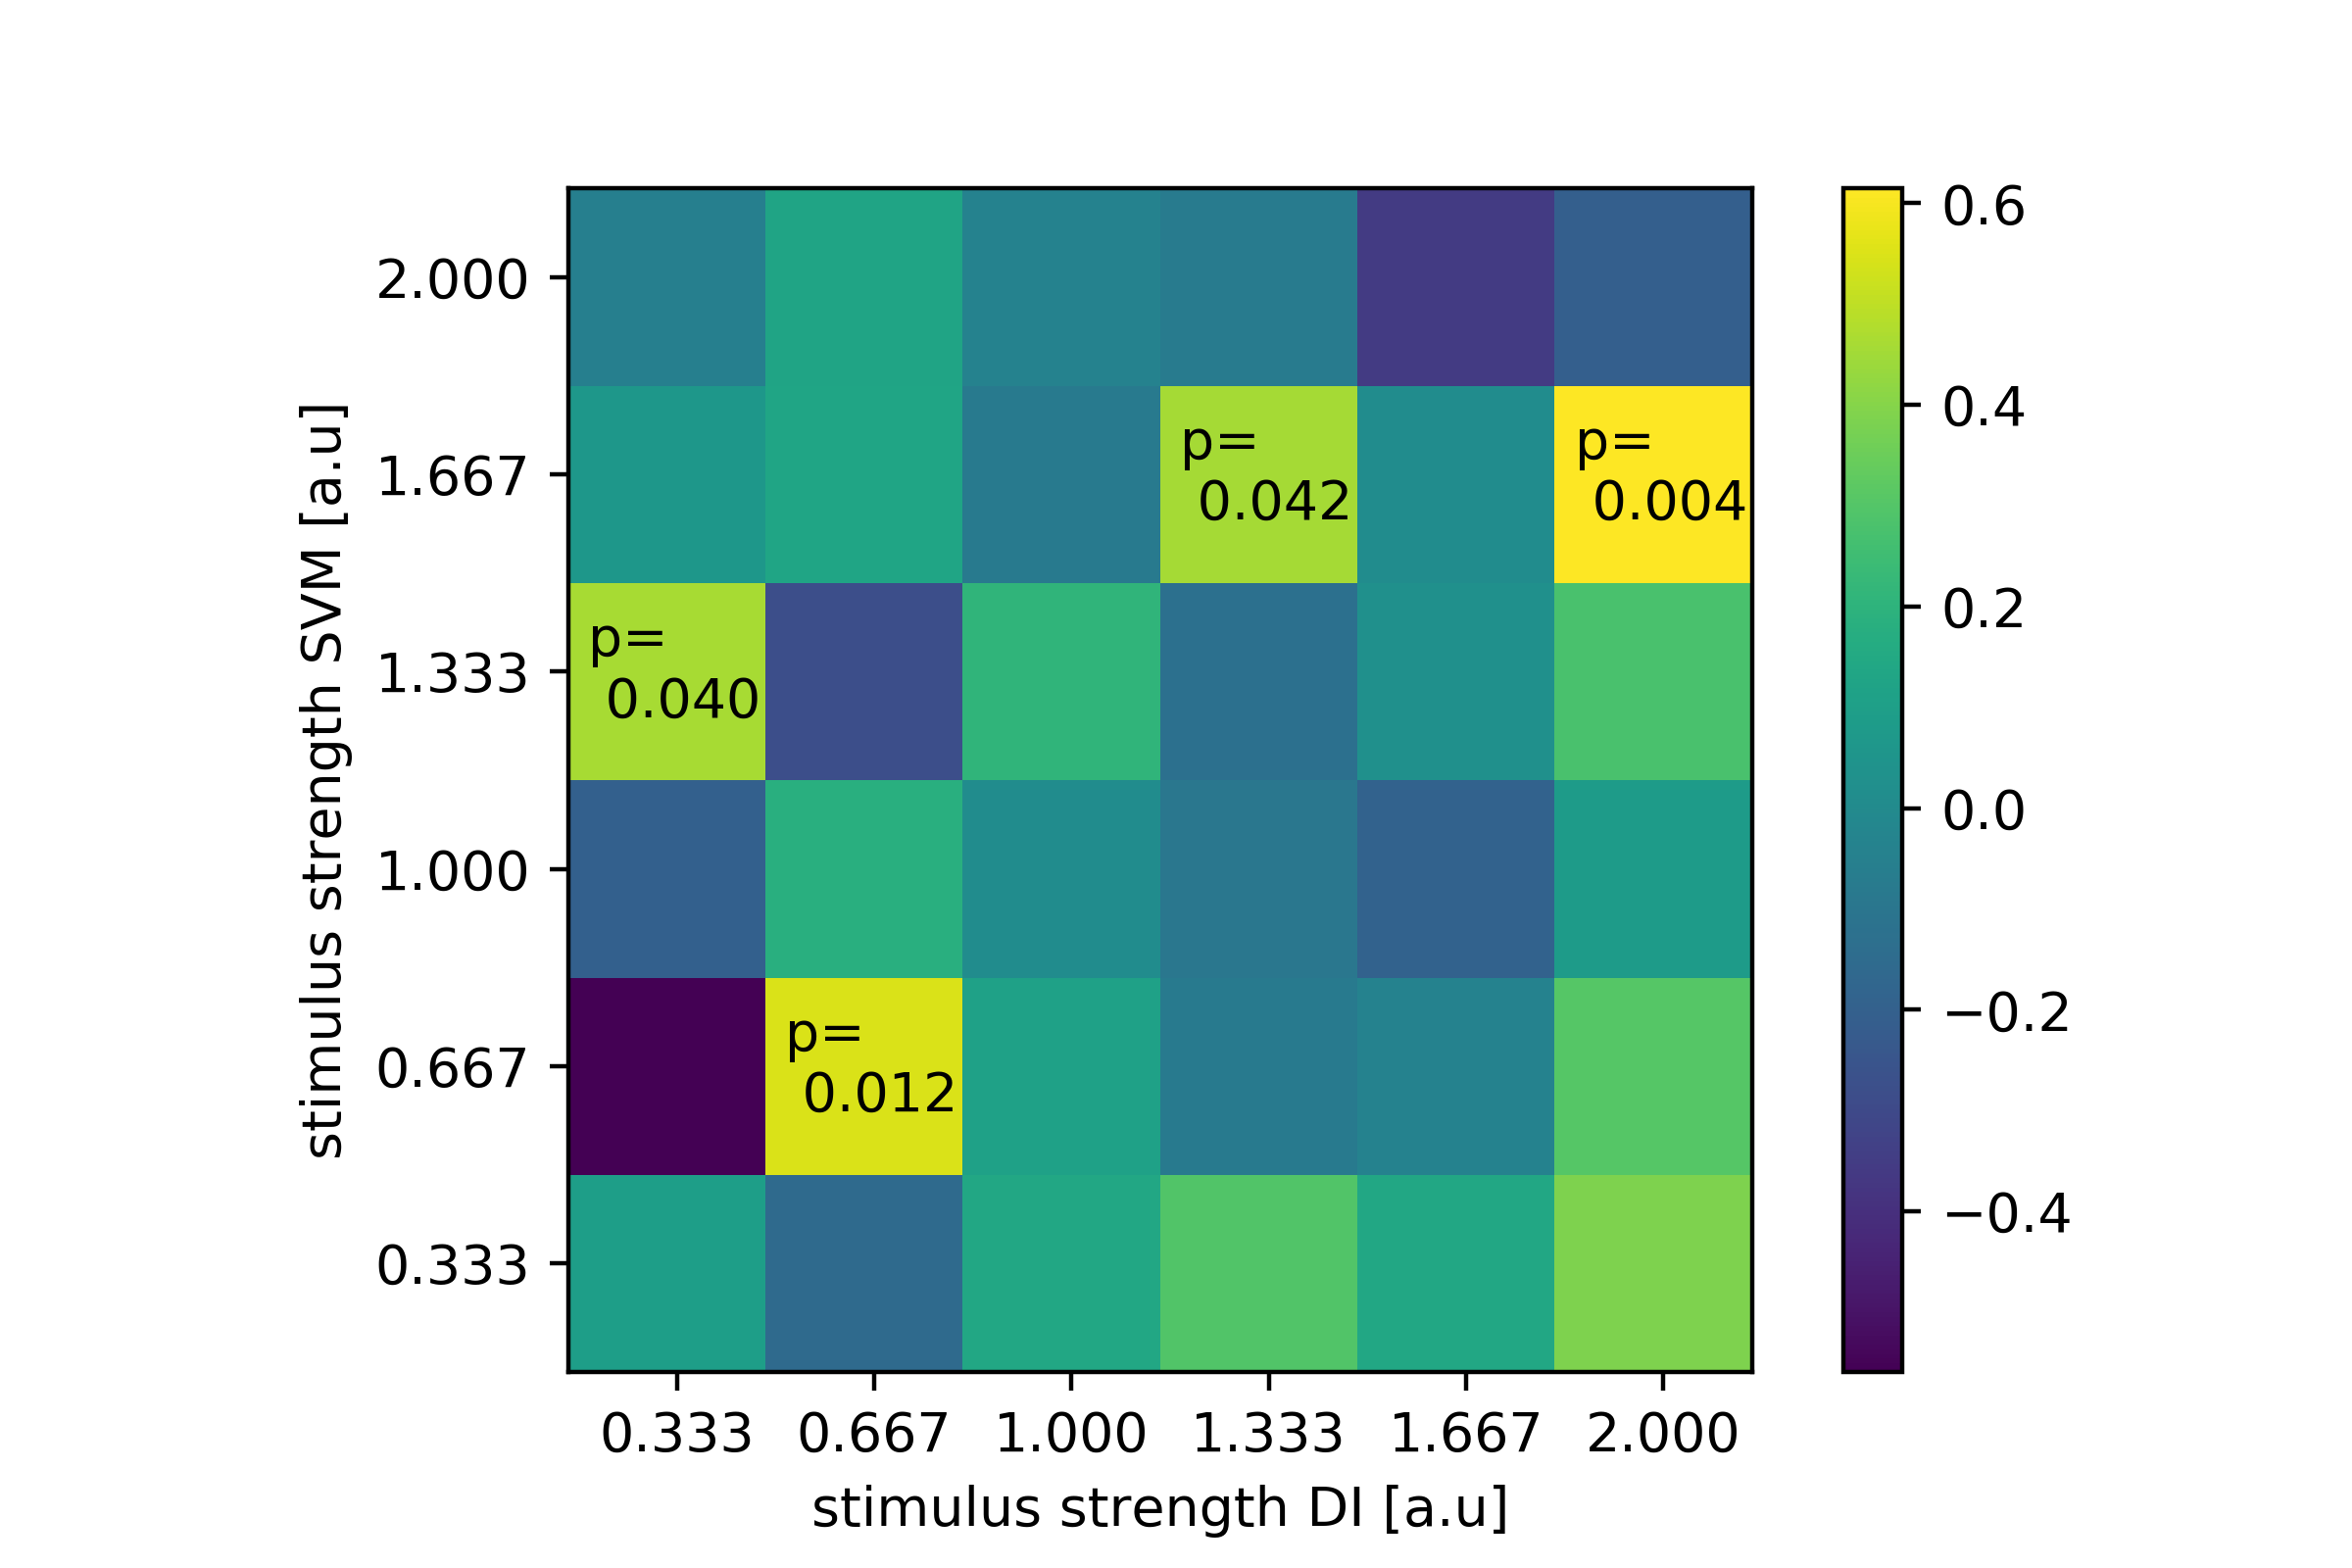
\includegraphics[width=1.0\textwidth]{DI_vs_SVM.png}
	\end{figure}
	\end{center}
\end{frame}

\begin{frame}[fragile]{Tuning Curves}
\begin{center}
	\begin{figure}
      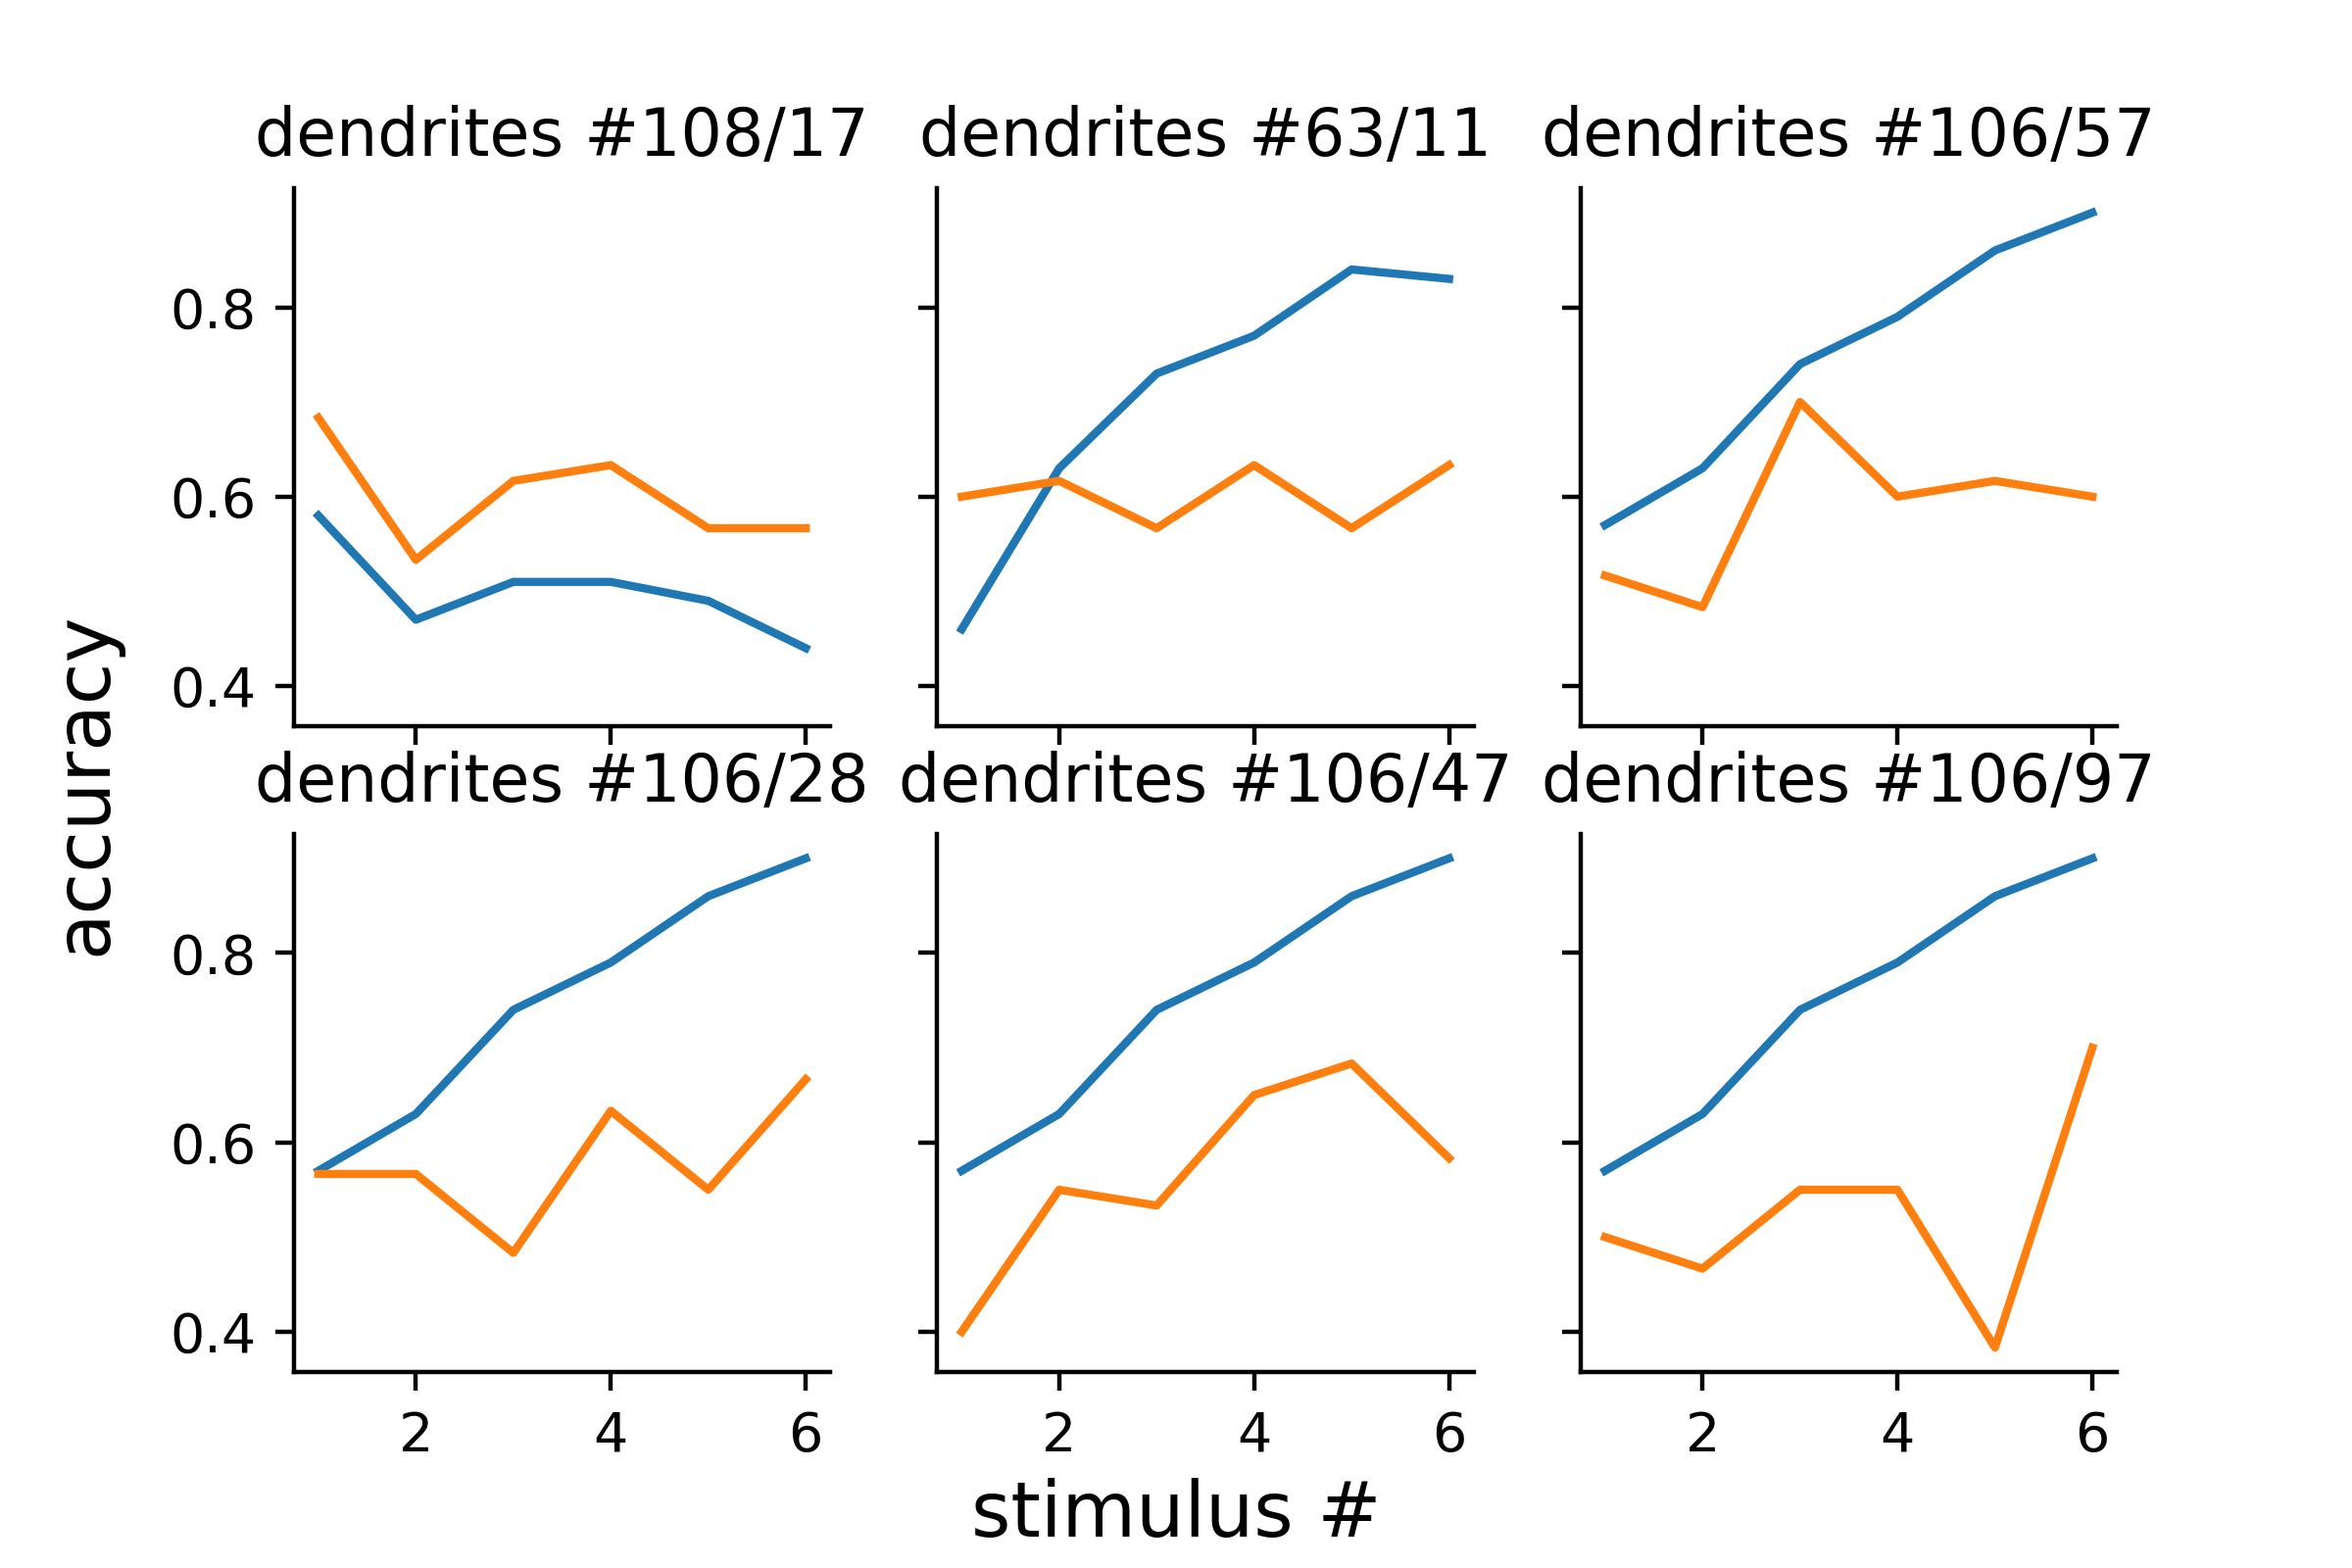
\includegraphics[width=1.0\textwidth]{tuning.png}
	\end{figure}
	\end{center}
\end{frame}

\begin{frame}[fragile]{Tuning Curves}
\begin{center}
	\begin{figure}
      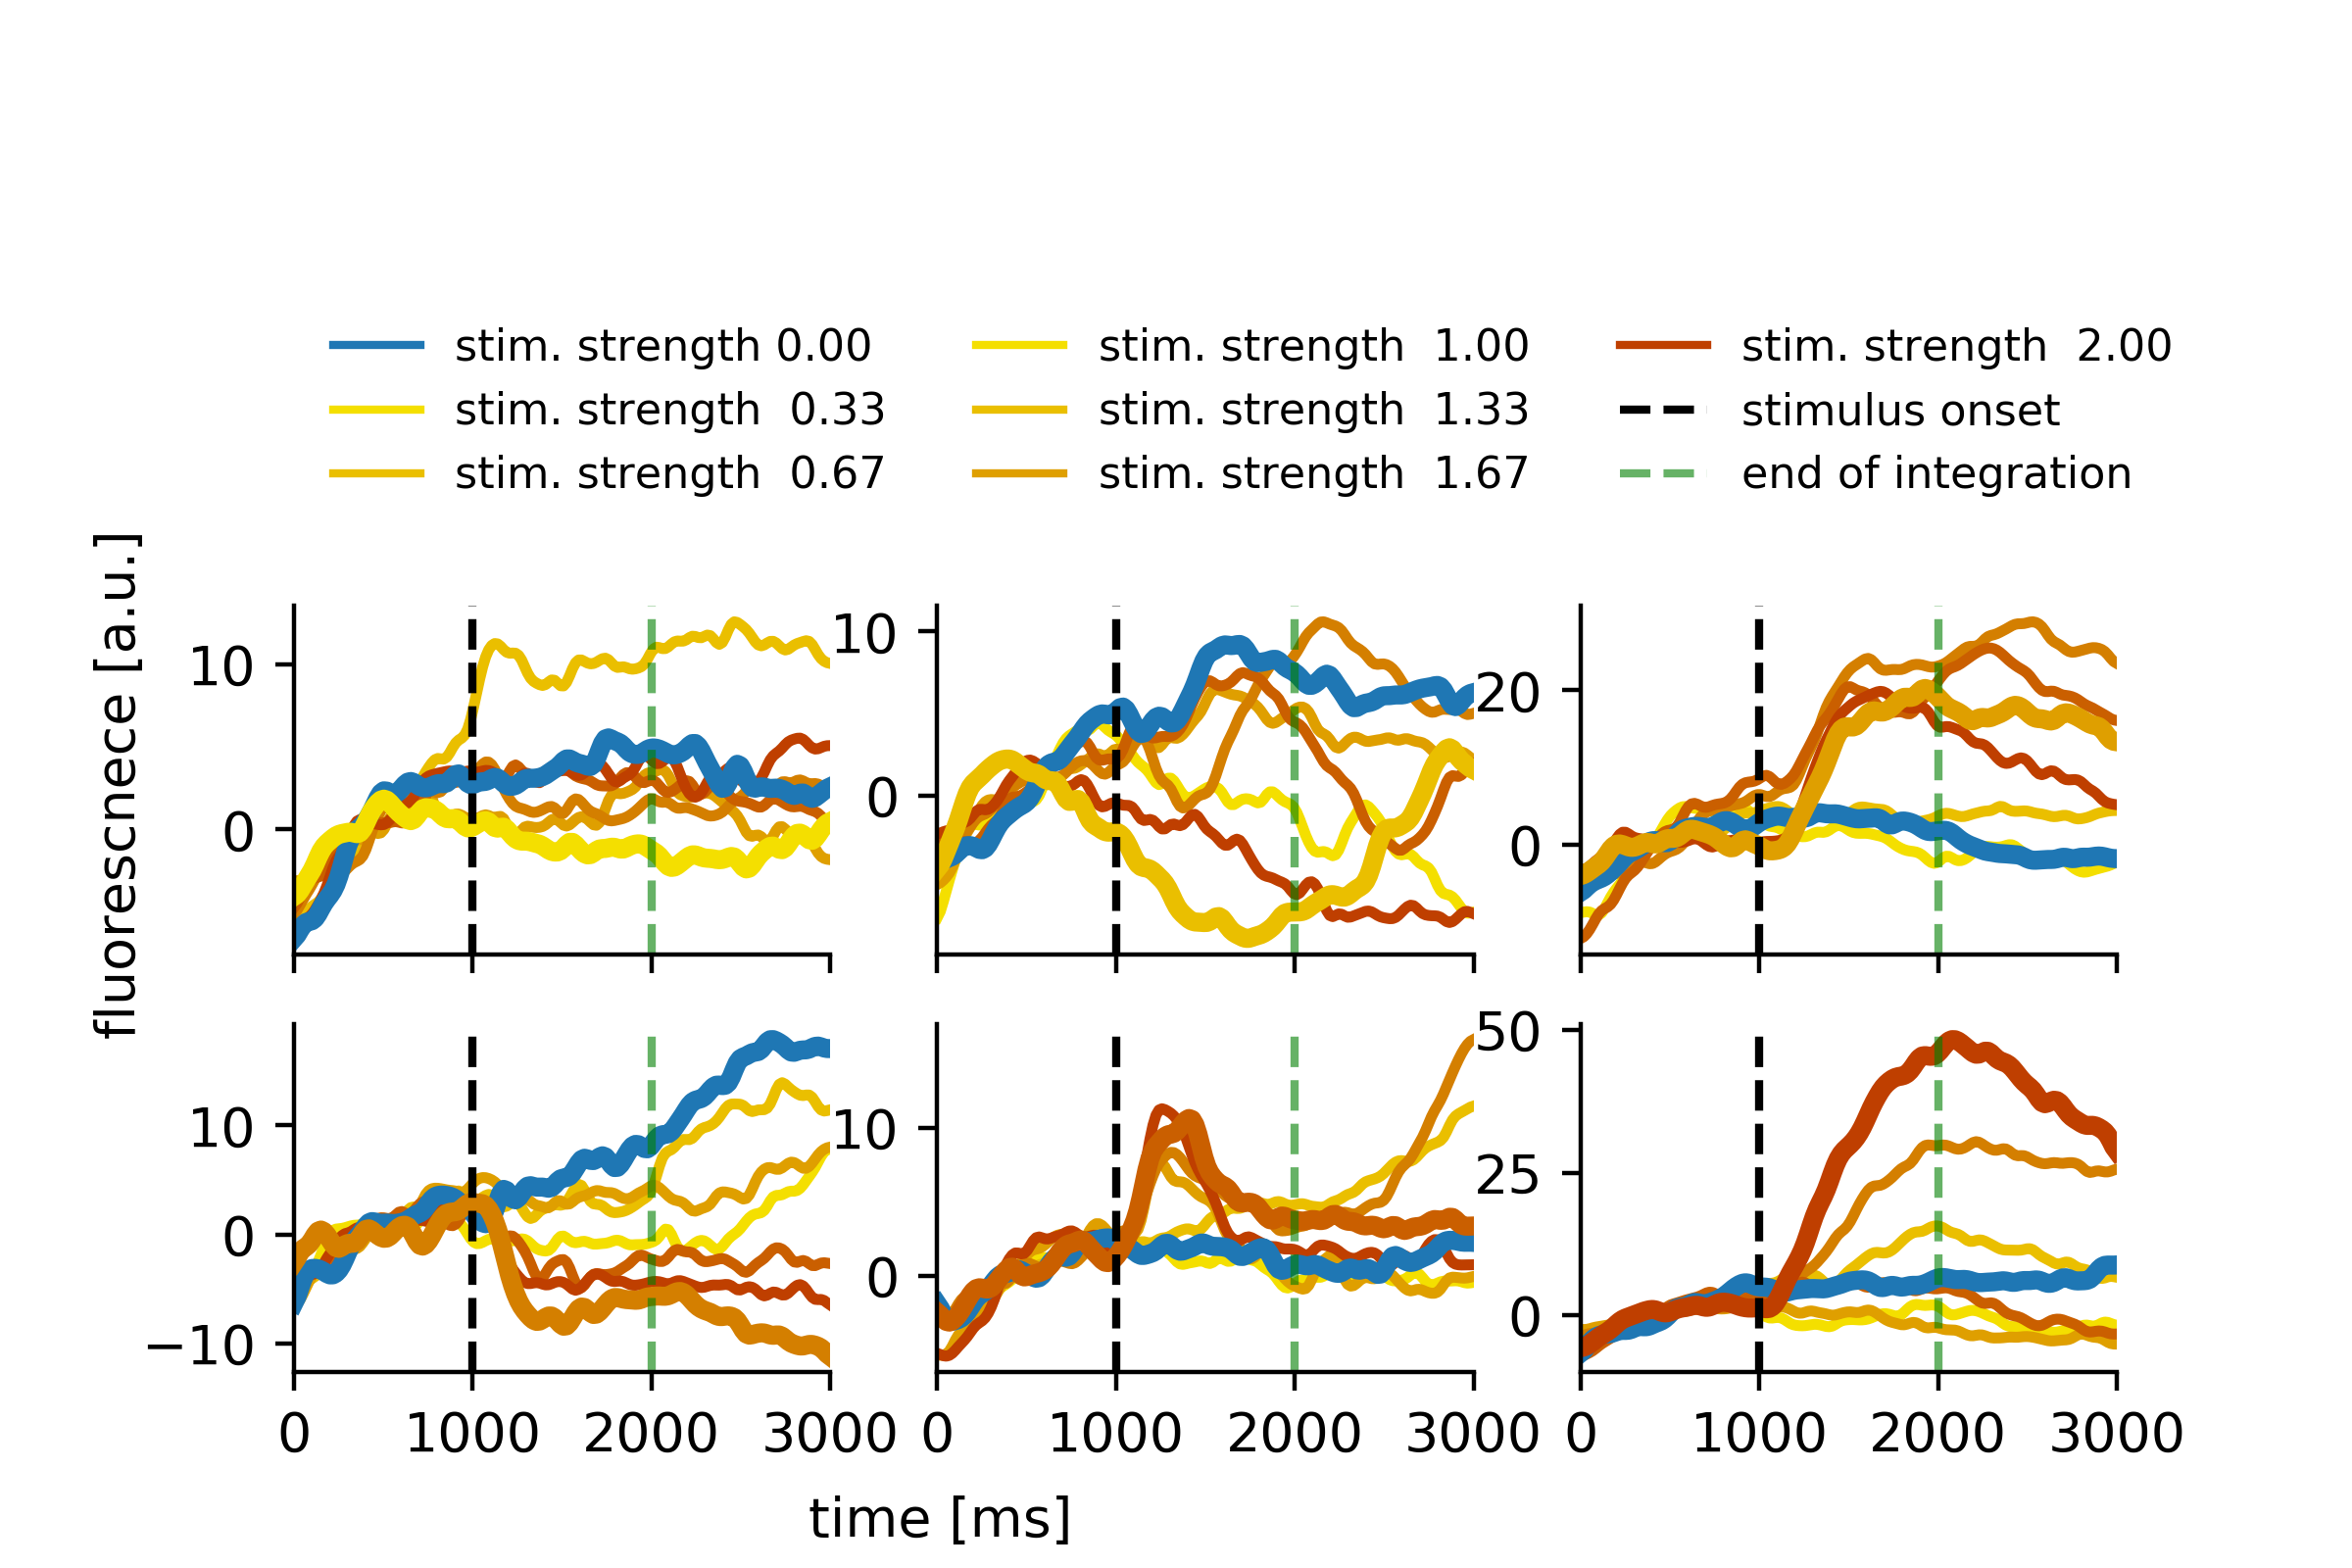
\includegraphics[width=1.0\textwidth]{tuning_ca2+.png}
      \caption*{todo:accuracies}
	\end{figure}
	\end{center}
\end{frame}

\begin{frame}[fragile]{Behavoreal Prediction - Most Accurate Dendrites}
\begin{table}
    \caption*{Stimulus strength 1 (near thereshold)}
    \begin{tabular}{c|c|c}
      \toprule
      Dendrite \# & Mean Accuracy & Standard Deviation\\
      \midrule
      70 & 0.78 & +/- 0.28\\
      47 & 0.77 & +/- 0.32\\
      56 & 0.73 & +/- 0.24\\
      92 & 0.70 & +/- 0.33\\
      \bottomrule
    \end{tabular}
  \end{table}
\end{frame}

\begin{frame}[fragile]{Behavoreal Tuning}
\begin{center}
	\begin{figure}
      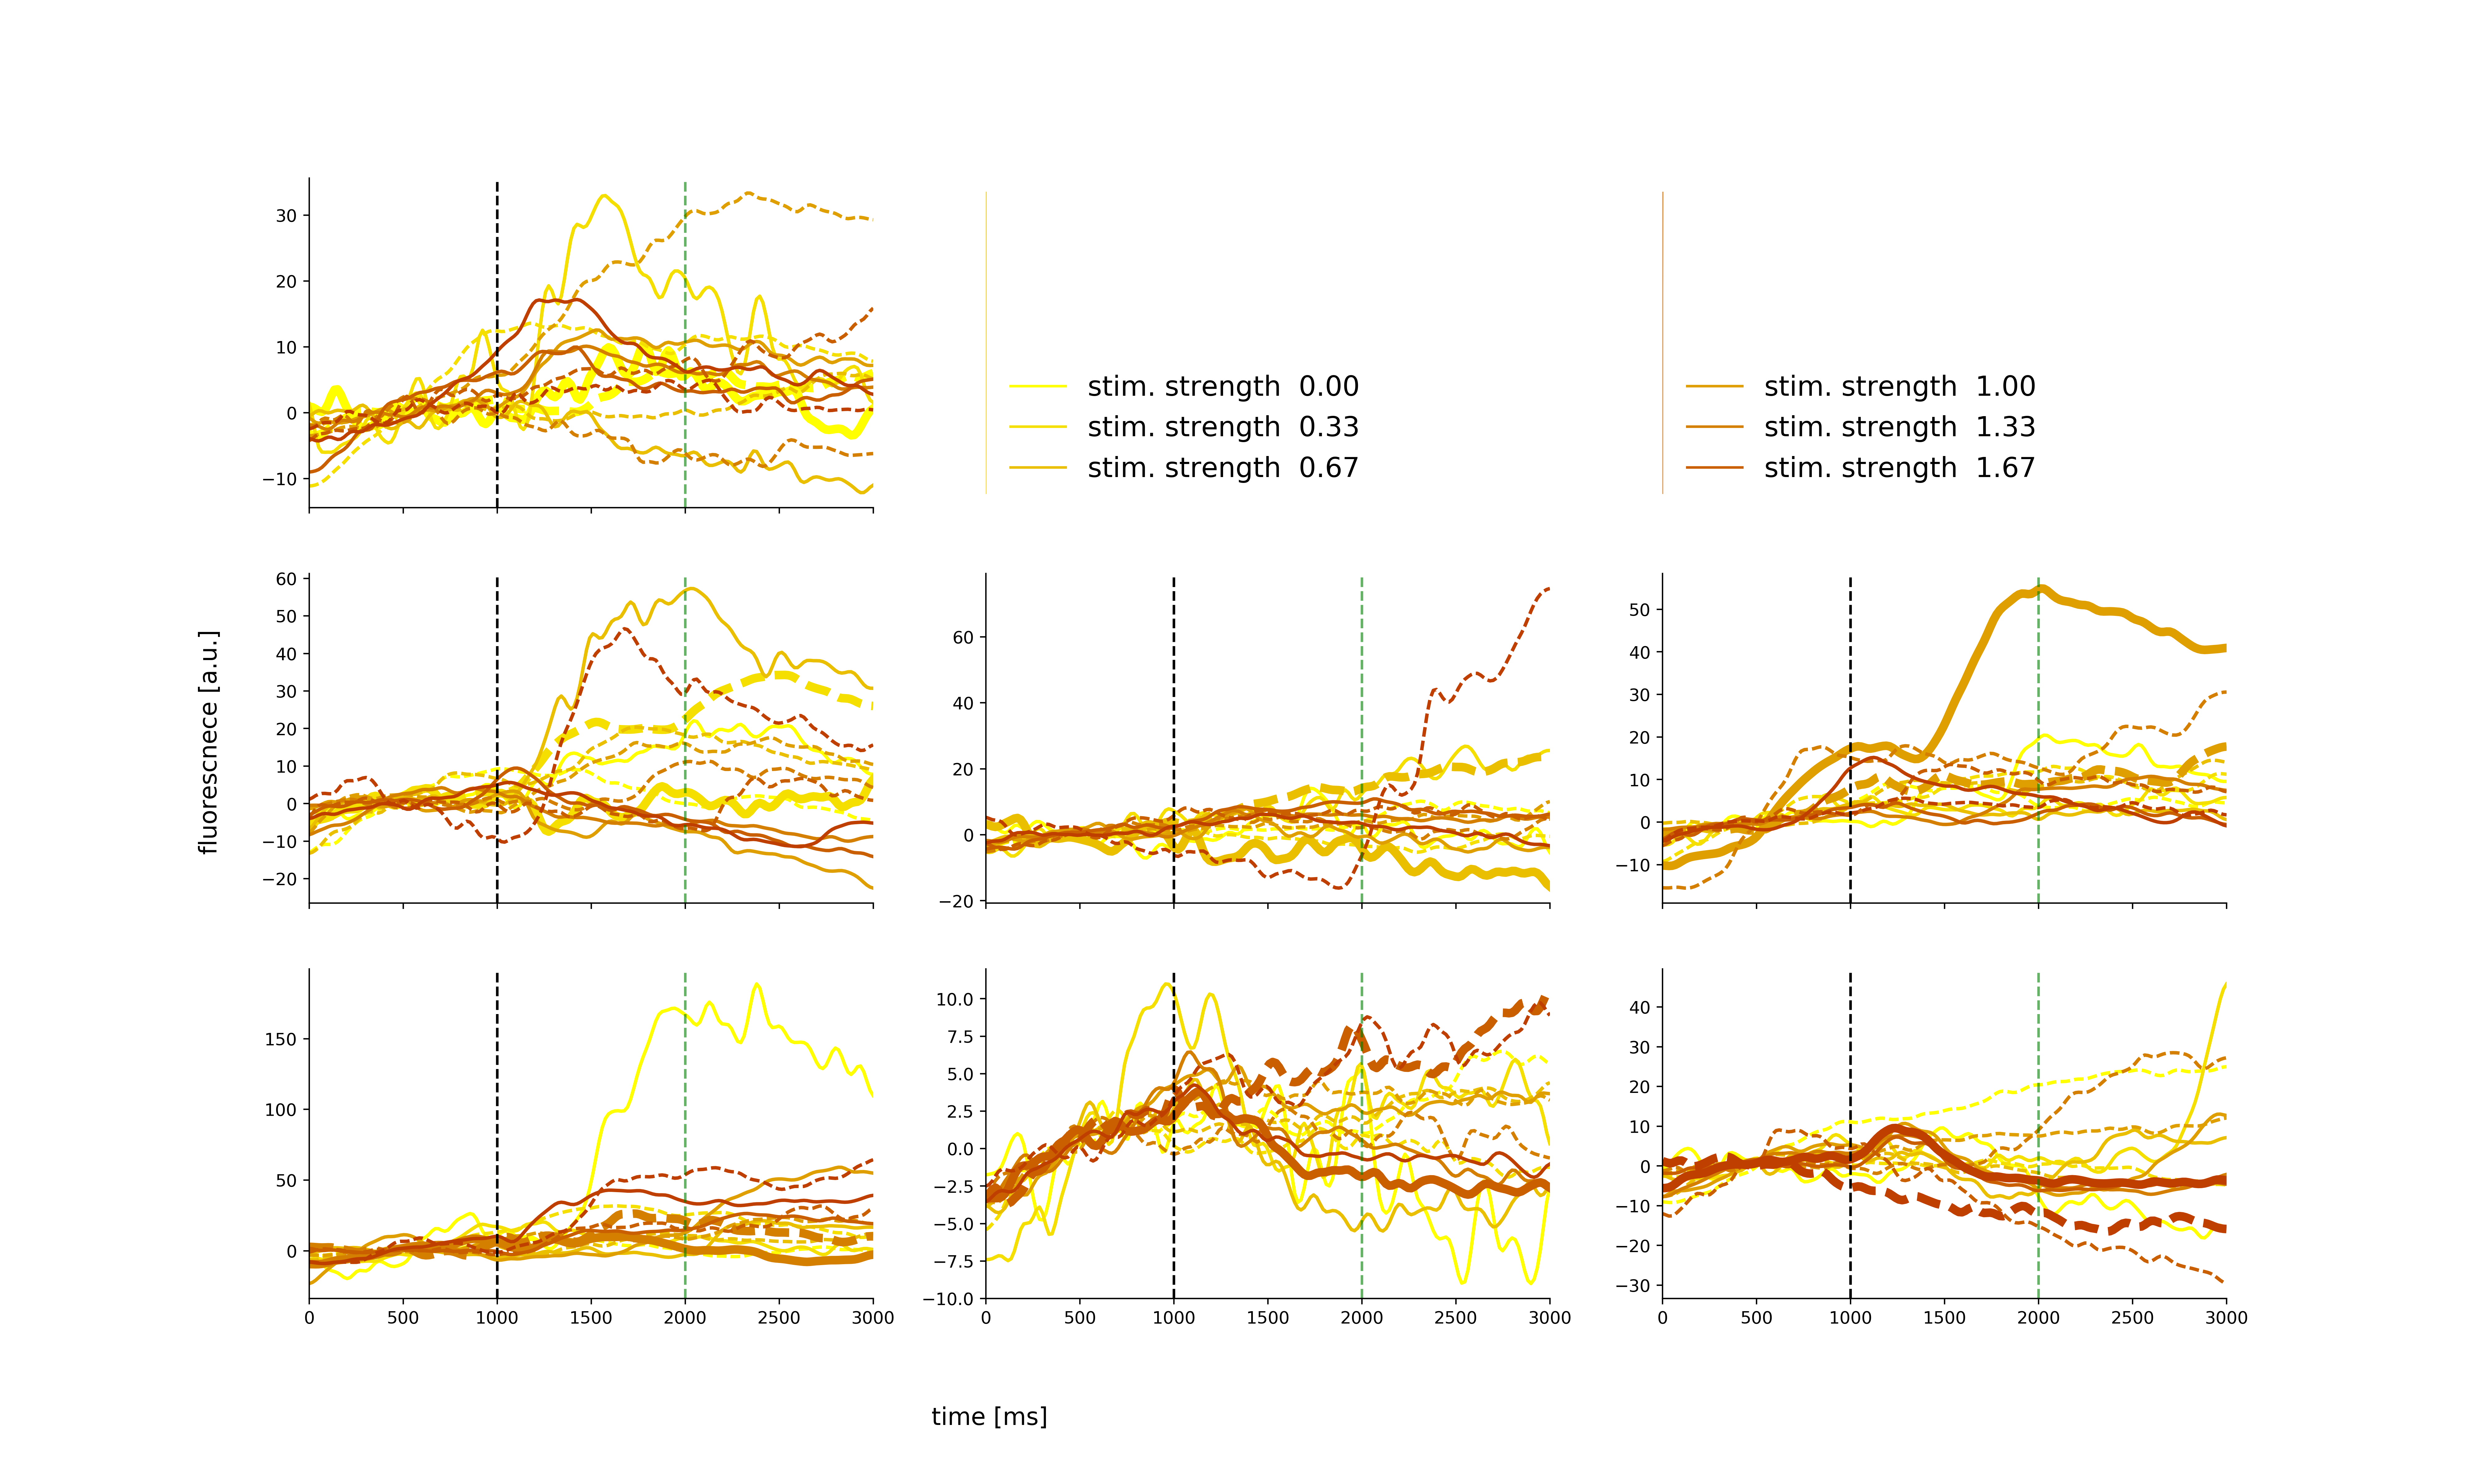
\includegraphics[width=1.0\textwidth]{tuning_ca2+_bb.png}
      \caption*{todo:accuracies}
	\end{figure}
	\end{center}
\end{frame}

\begin{frame}[fragile]{Rank Correlations of Behavoreal and Presence Dendrites}
\begin{center}
	\begin{figure}
	\caption*{reduce ndends}
      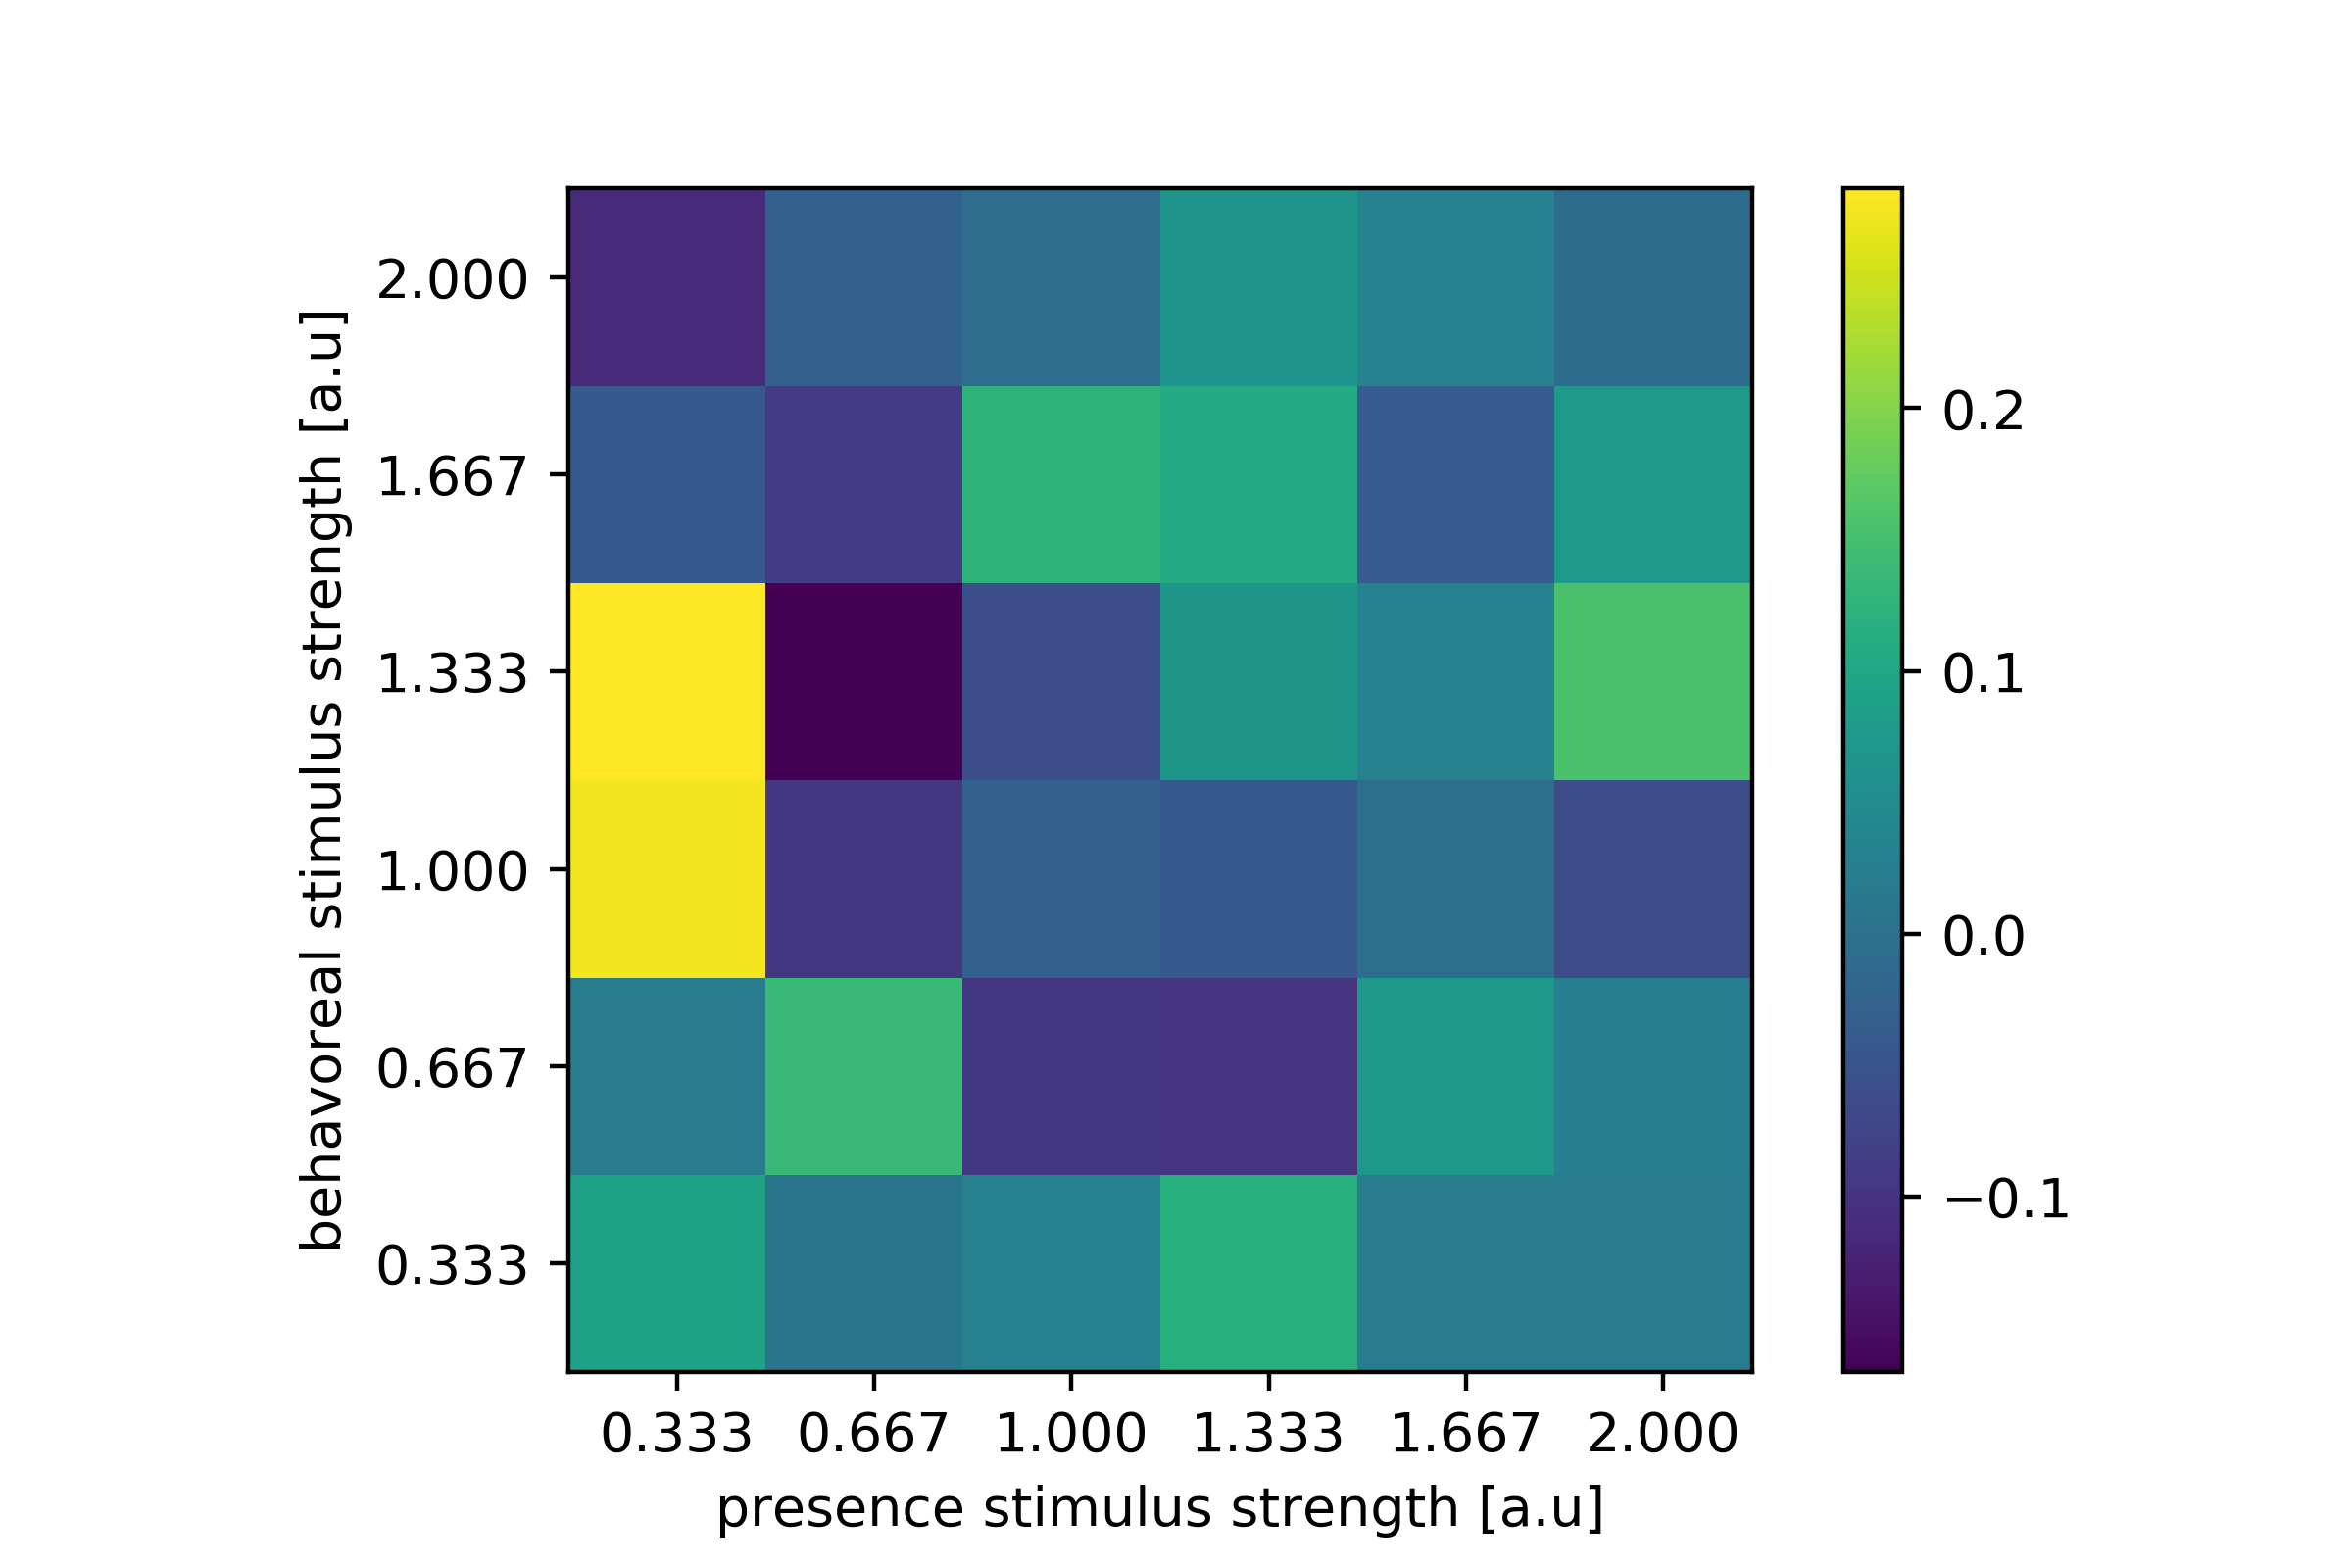
\includegraphics[width=1.0\textwidth]{transrank.png}
	\end{figure}
	\end{center}
\end{frame}

\section{Multivariate SMV Analysis}

\begin{frame}[fragile]{SVM Performance on Combined Dendrites}
Placeholder - Something wrong when using other files!
\end{frame}

\begin{frame}[fragile]{SVM Performance on Combined Dendrites - Behavoreal}
Placeholder - Something wrong when using other files!
\end{frame}

\begin{frame}[fragile]{Optimal Averaging Times}
\begin{center}
	\begin{figure}
	\caption*{Solve Problem with combined SVM first}
      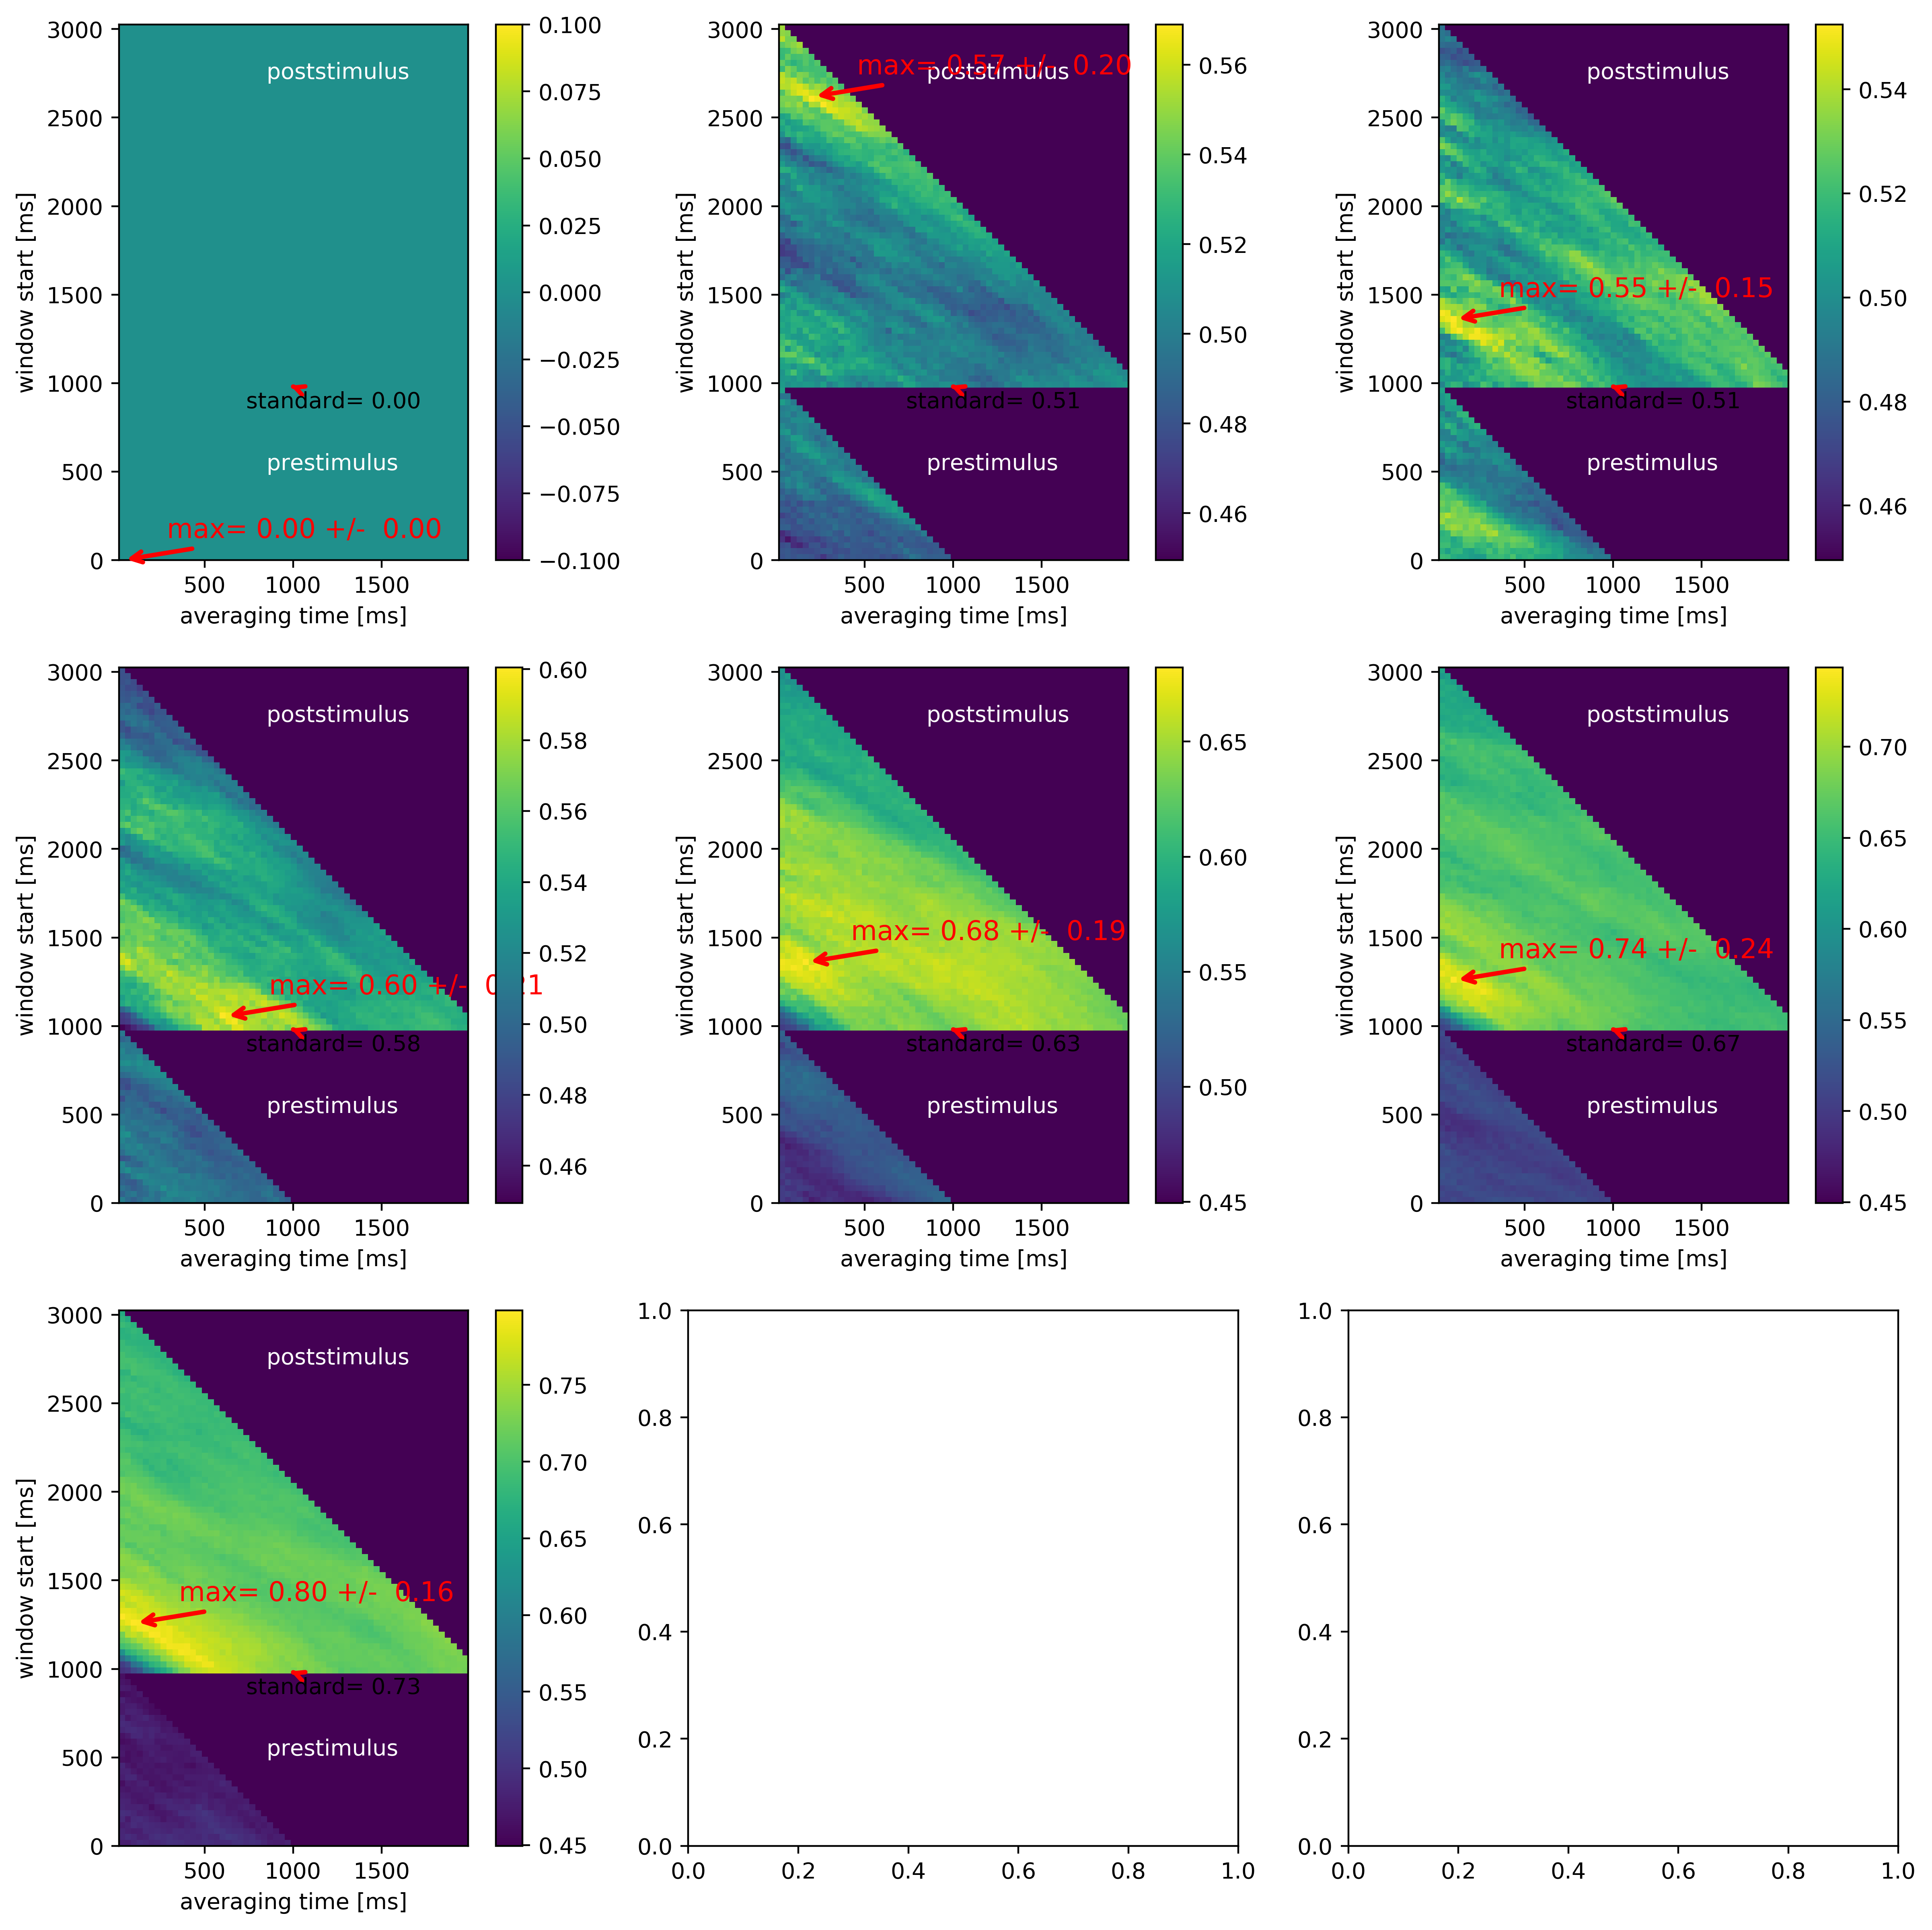
\includegraphics[width=1.0\textwidth]{placeholder_wind_pres.png}
	\end{figure}
	\end{center}
\end{frame}

\begin{frame}[fragile]{Optimal Averaging Times - Behavior}
\begin{center}
	\begin{figure}
	\caption*{Solve Problem with combined SVM first}
      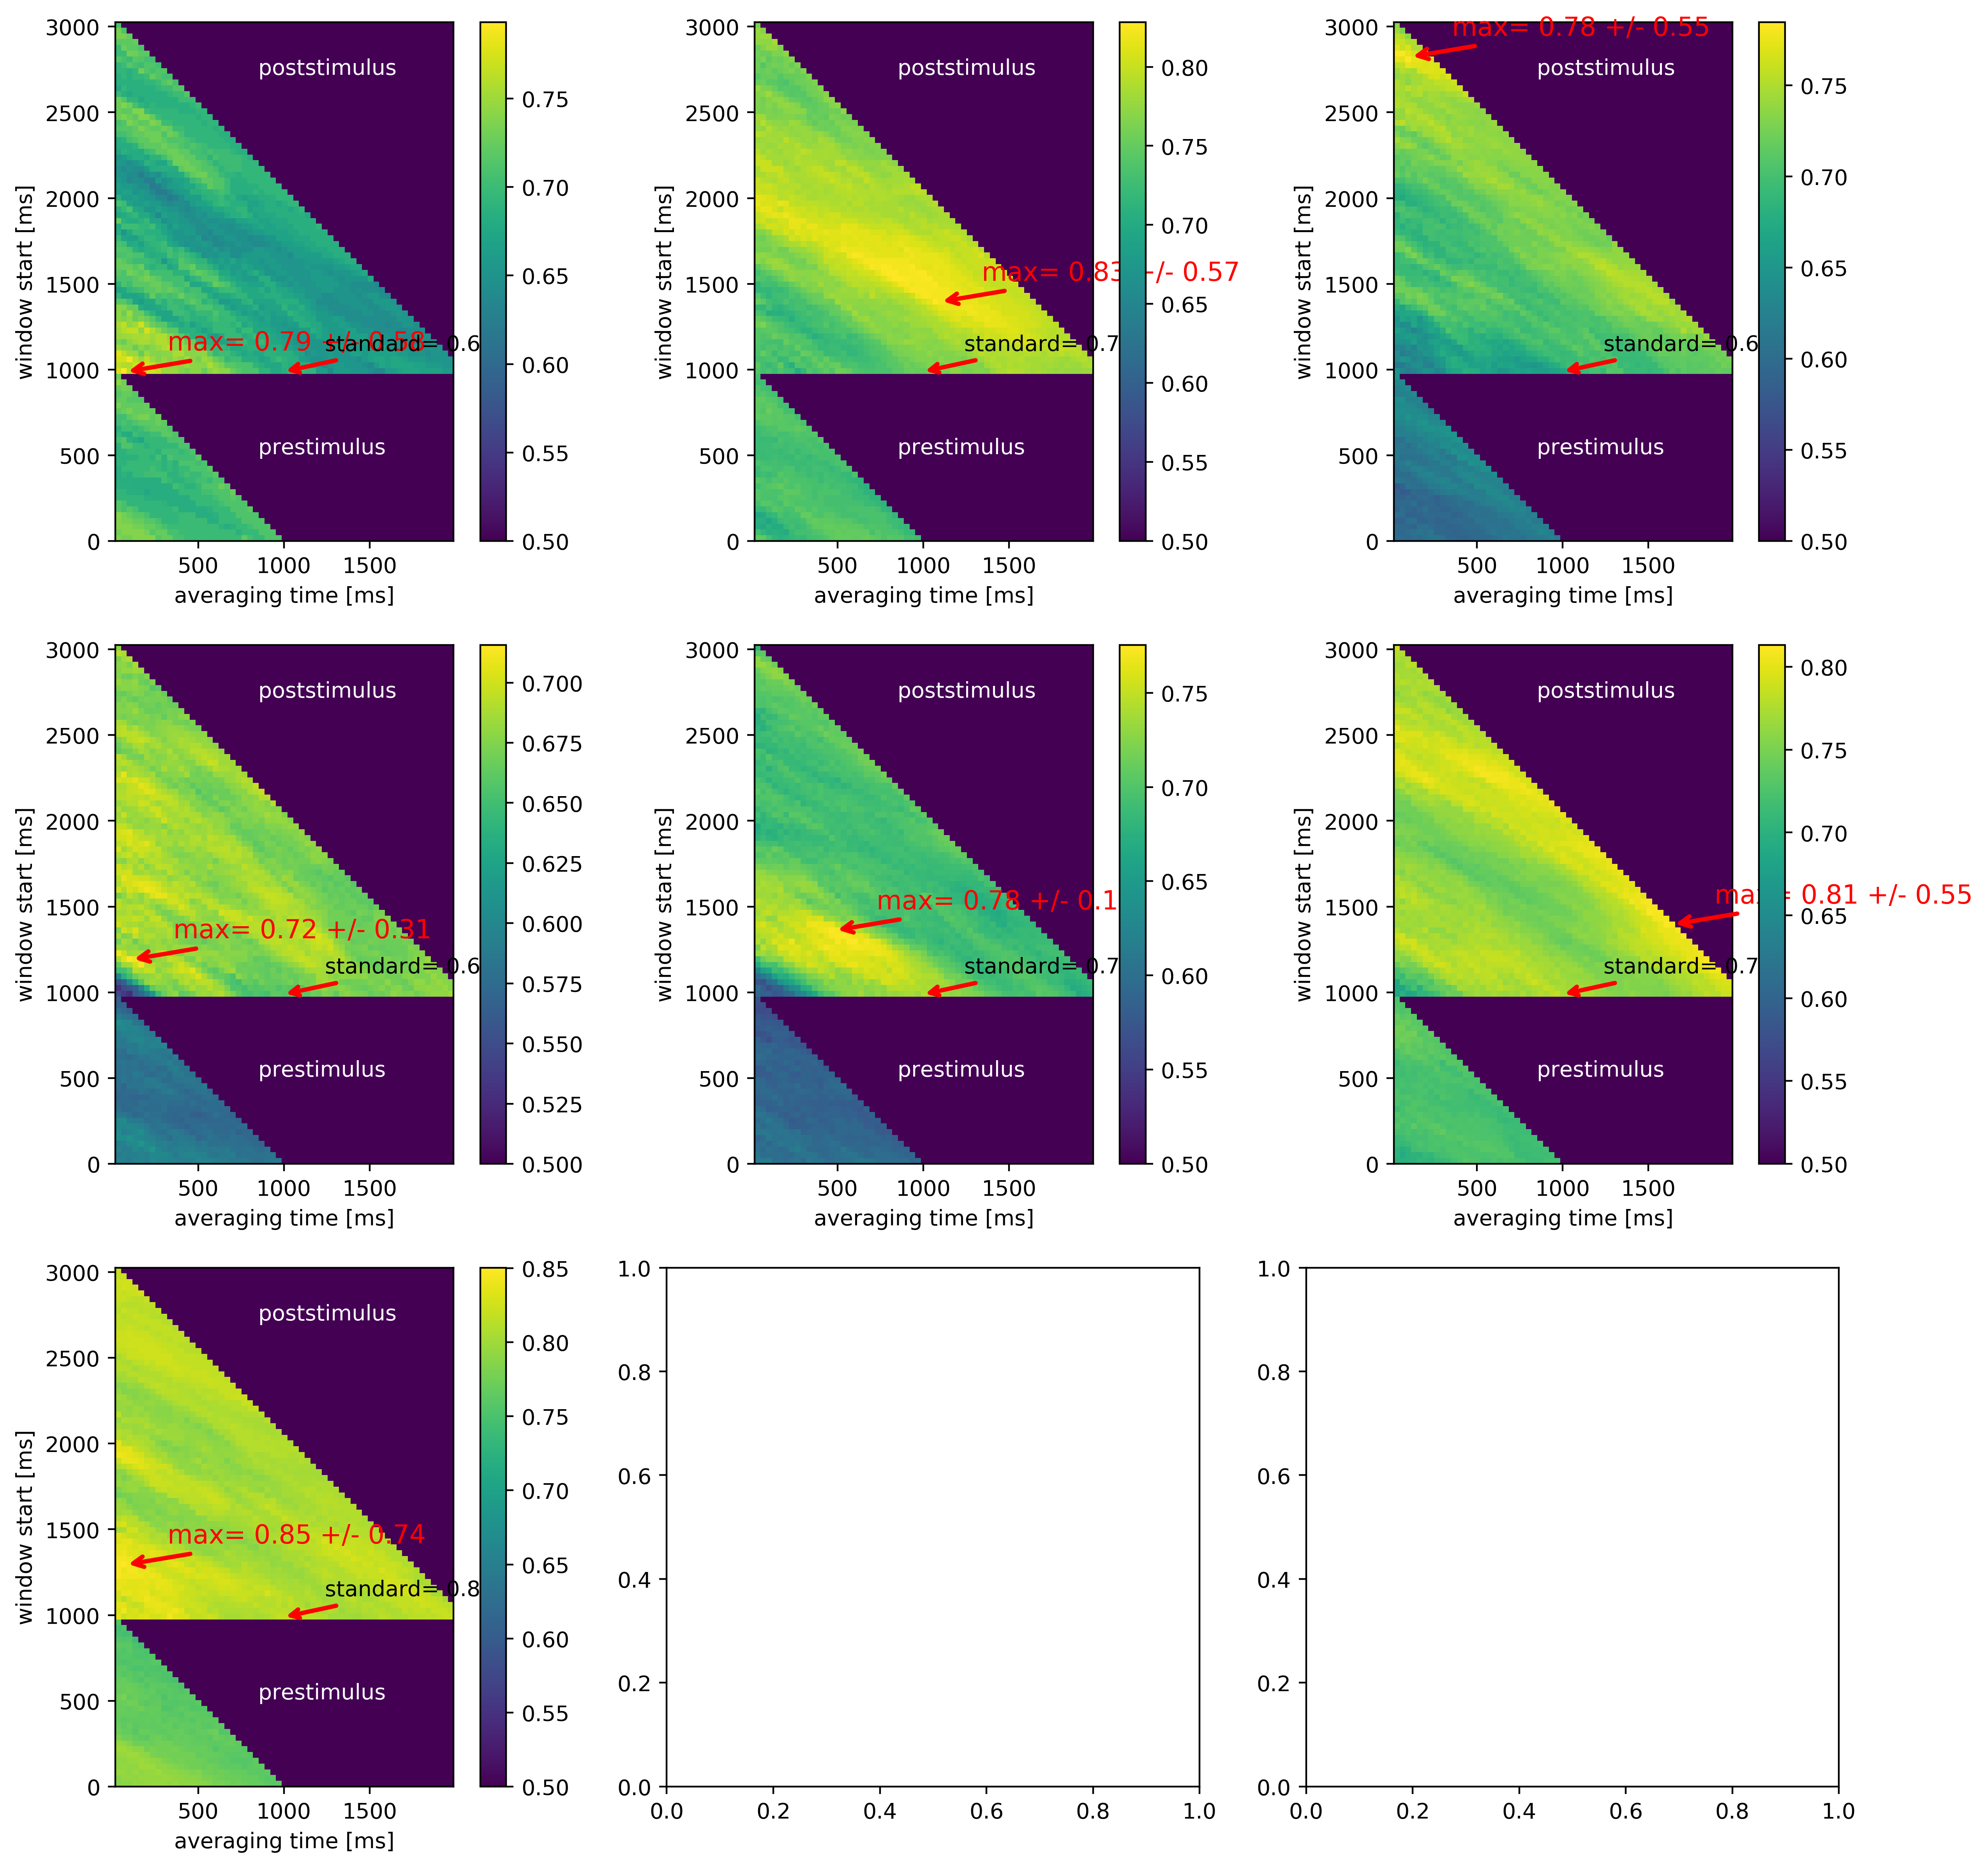
\includegraphics[width=1.0\textwidth]{placeholder_wind_hit.png}
	\end{figure}
	\end{center}
\end{frame}

\begin{frame}[fragile]{Mante - Approach (Placeholder Title)}
Math goes here
\end{frame}

\begin{frame}[fragile]{Mante - Approach - Results}
\begin{center}
	\begin{figure}
	\caption*{Solve Problem with combined SVM first}
      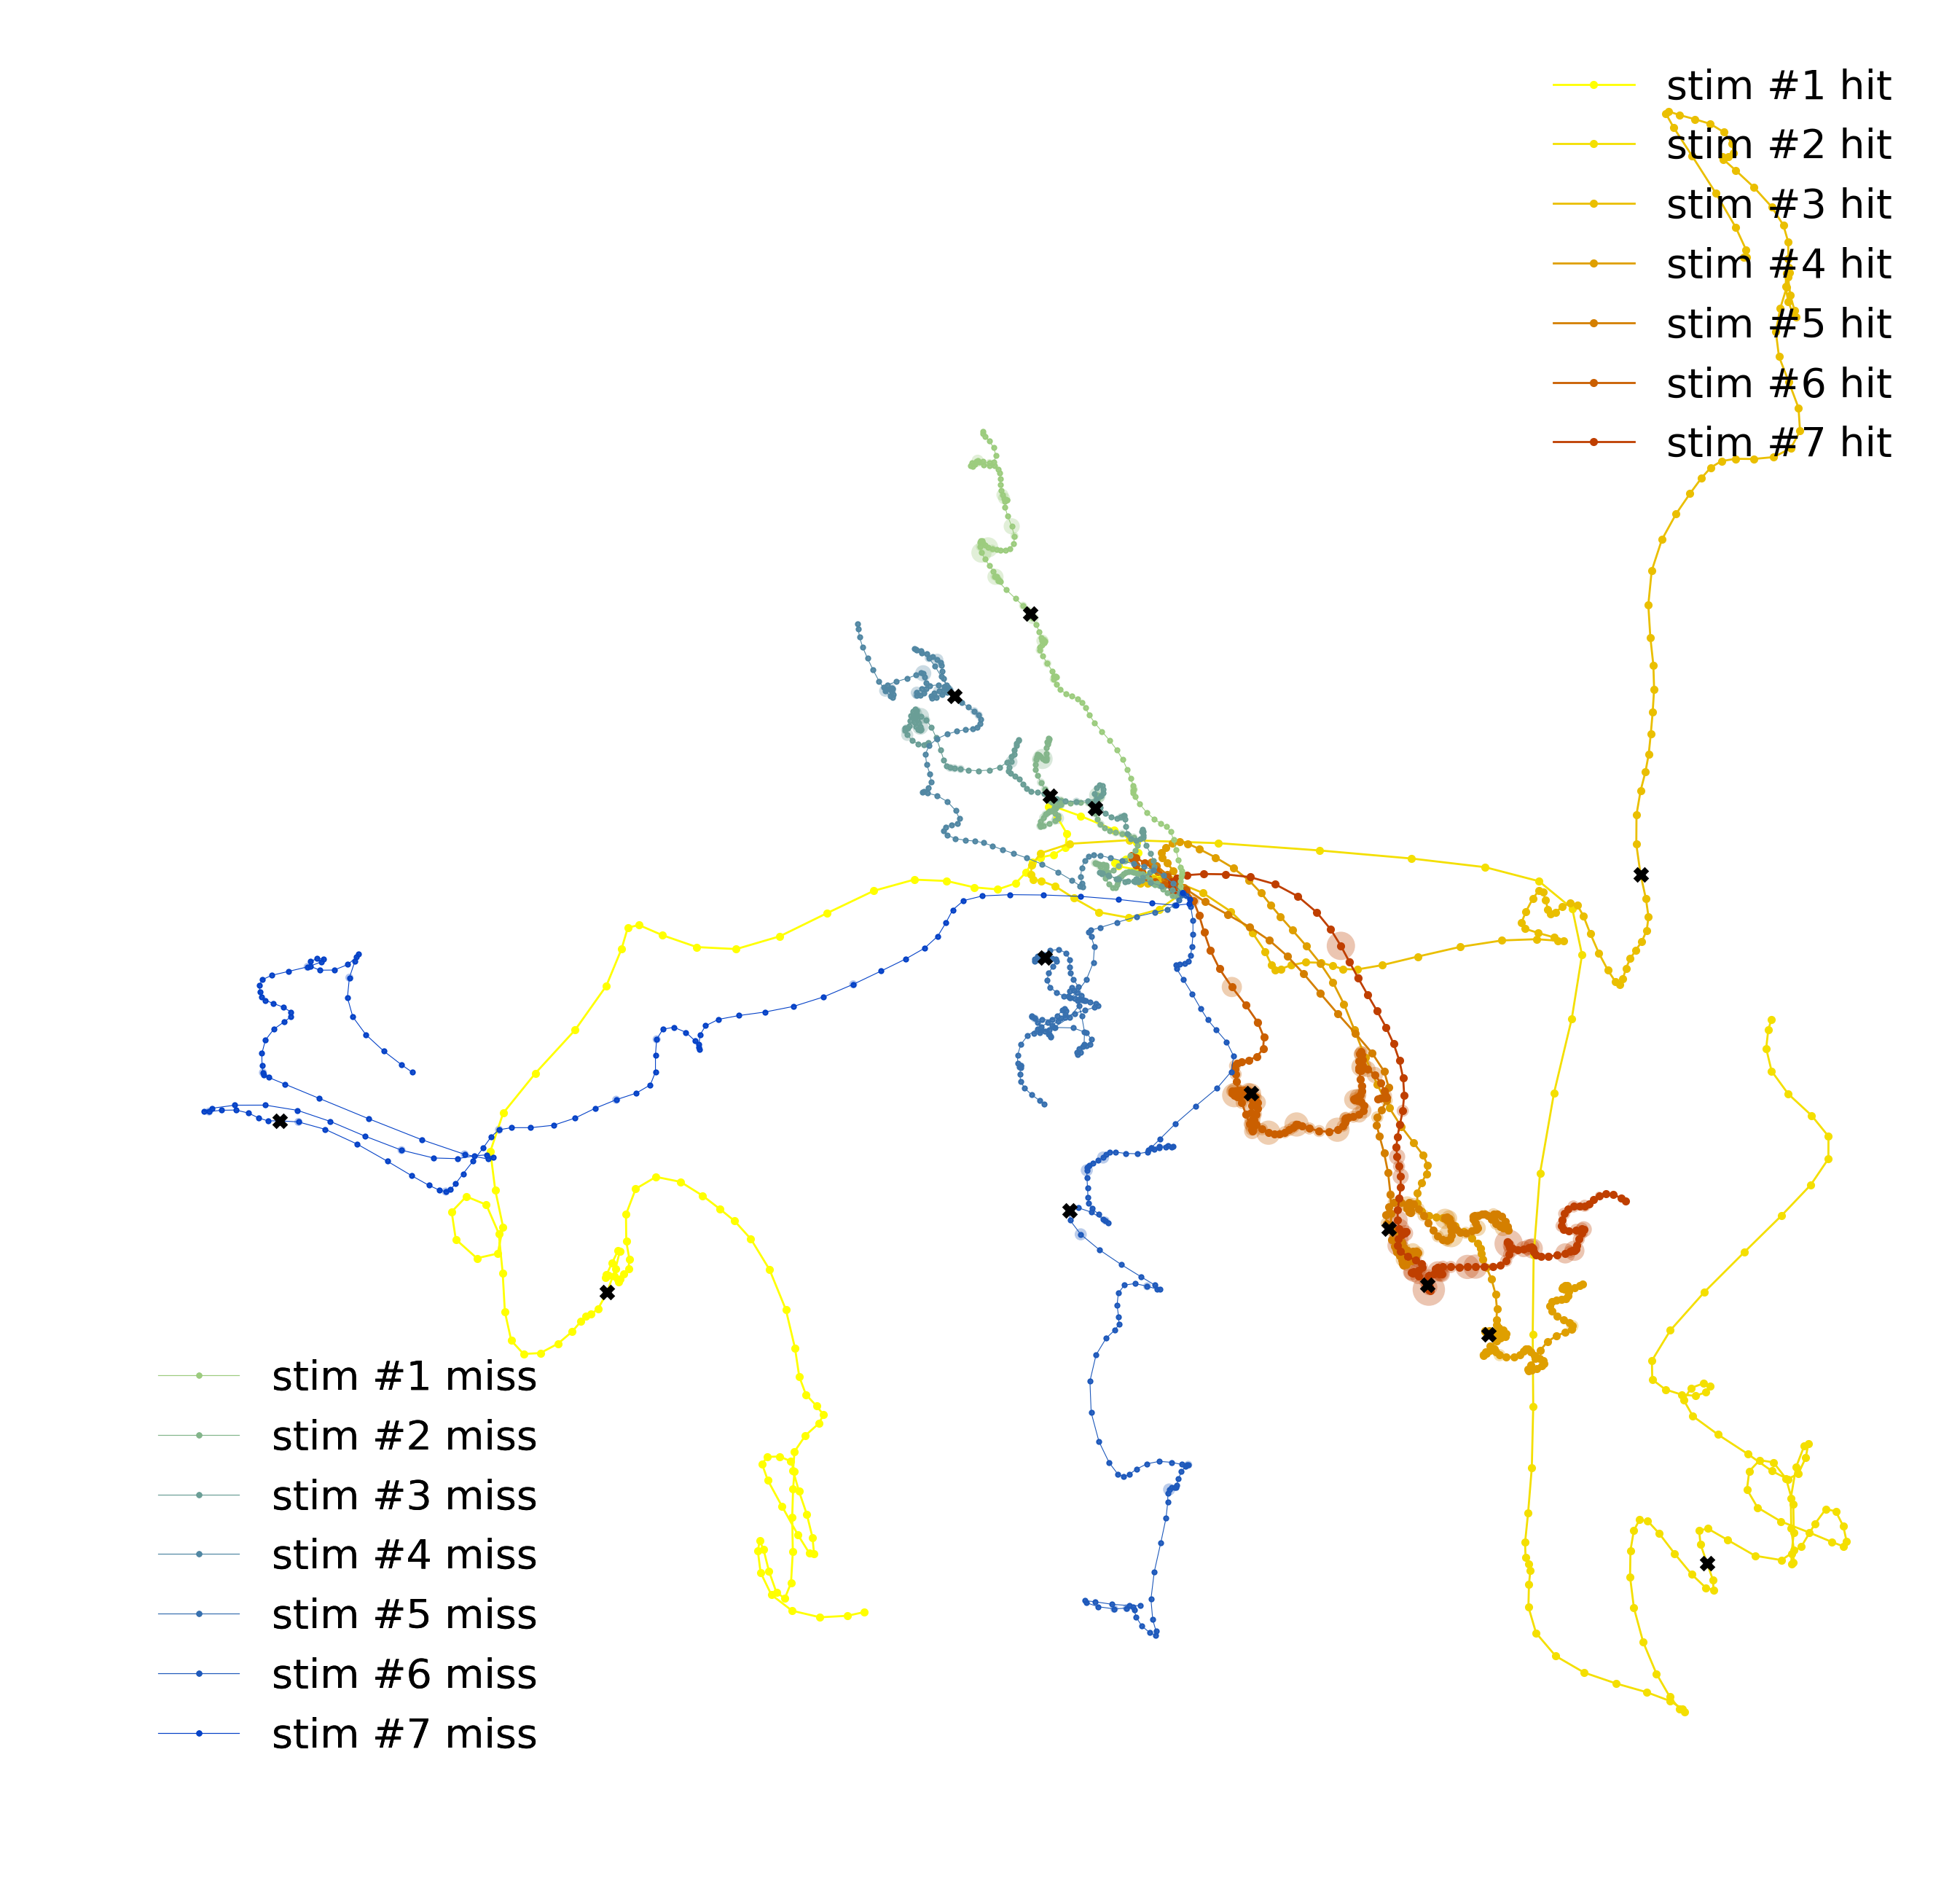
\includegraphics[width=1.0\textwidth]{reg_norm_placeholder.png}
	\end{figure}
	\end{center}
\end{frame}

\begin{frame}[fragile]{Mante - Approach - Results}
\begin{center}
	\begin{figure}
	\caption*{Solve Problem with combined SVM first}
      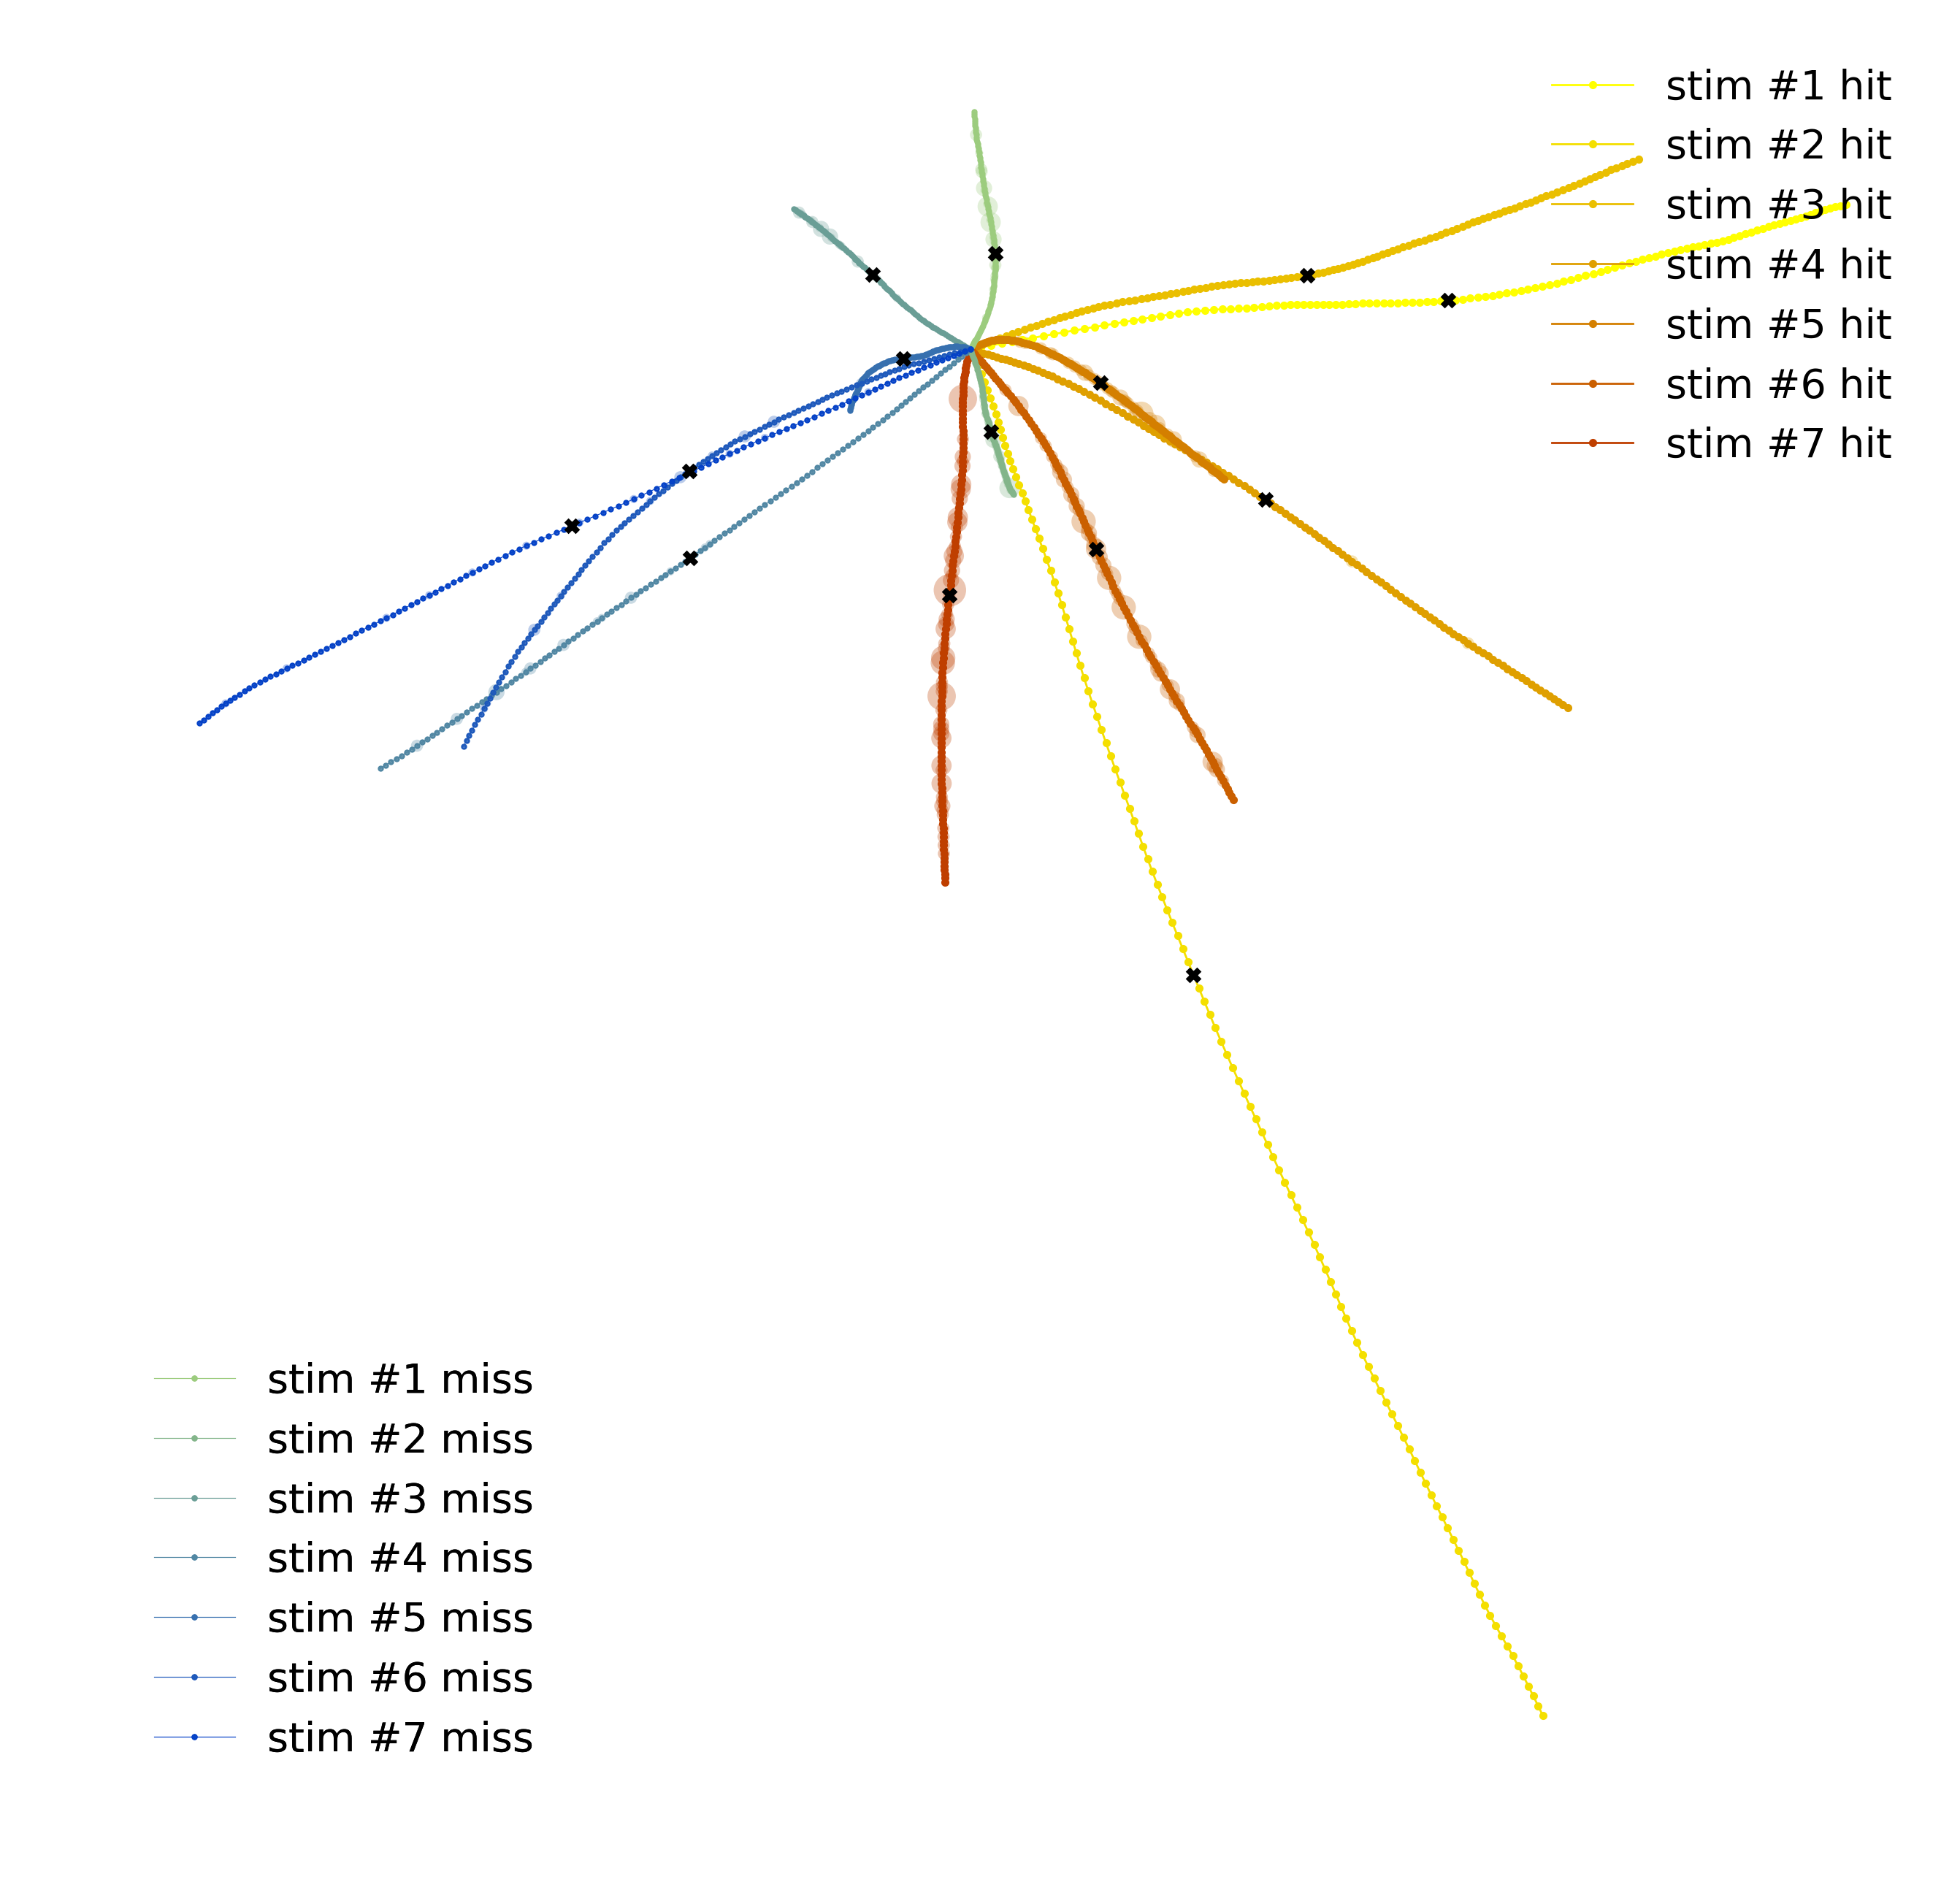
\includegraphics[width=1.0\textwidth]{reg_inte_placeholder.png}
	\end{figure}
	\end{center}
\end{frame}

\end{document}
